\documentclass[
fontsize=10pt, 
listof = totoc,
parskip = half	
]{report}
\usepackage[utf8]{inputenc}
\usepackage[german]{babel}
\usepackage[fixlanguage]{babelbib}
\selectbiblanguage{german}
\usepackage[dvipsnames, table]{xcolor}
\usepackage{colortbl}
\usepackage[most]{tcolorbox}
\usepackage[]{acronym}
\usepackage[T1]{fontenc}
\usepackage[absolute]{textpos}
\usepackage{amsmath}
\usepackage{amsthm}
\usepackage{amsfonts}
\usepackage[ruled,vlined,linesnumbered,ngerman]{algorithm2e}
\usepackage{tabu}
\usepackage{graphicx}
\usepackage{mdframed}
\usepackage{float}
\usepackage{lipsum}
\usepackage{fontawesome}  
\usepackage{esvect}
\usepackage{booktabs} % table style
\usepackage{tabularx}
\usepackage{multirow} % table style
\usepackage{amssymb}
\usepackage{nicefrac}
\usepackage{cancel}
\usepackage{polynom}
\usepackage{stmaryrd} 
\usepackage{caption}
\usepackage{subcaption}
\usepackage{paralist}
% for graphics
\usepackage{physics}
\usepackage{amsmath}
\usepackage{tikz}
\usepackage{mathdots}
\usepackage{yhmath}
\usepackage{cancel}

\usepackage{chngcntr}
%\counterwithout{figure}{chapter}
%\counterwithout{table}{chapter}

\usepackage[hidelinks, plainpages=false, pdfpagelabels]{hyperref}


\newenvironment{tableEnum}{\begin{varwidth}[t]{\linewidth}\begin{compactenum}[1)]}{\end{compactenum}\end{varwidth}\vspace{0.08cm}}
\newenvironment{tableItem}{\begin{varwidth}[t]{\linewidth}\begin{compactitem}[-]}{\end{compactitem}\end{varwidth}\vspace{0.08cm}}

\usepackage[left=2cm,right=2cm,top=2cm,bottom=2cm]{geometry}
\author{Michael Kaip}

\date{}

% Extension for amsmath matrix environment - matrix | vector
\makeatletter
\renewcommand*\env@matrix[1][*\c@MaxMatrixCols c]{%
	\hskip -\arraycolsep
	\let\@ifnextchar\new@ifnextchar
	\array{#1}}
\makeatother

%Extension for roman numbers
\newcommand{\uproman}[1]{\uppercase\expandafter{\romannumeral#1}}
\newcommand{\lowroman}[1]{\romannumeral#1\relax}

\newtheorem{definition}{Definition}

\newenvironment{conditions}
{\par\vspace{\abovedisplayskip}\noindent\begin{tabular}{>{$}l<{$} @{${}:{}$} l}}
	{\end{tabular}\par\vspace{\belowdisplayskip}}


%%%%%%%%%%%%%%%%%%%%%%%%%%%%%%%%%%%%%%%%

\begin{document}
\begin{titlepage}
	\vspace*{-\headsep}\vspace{-\headheight}
	\noindent
	
\includegraphics[scale=0.38]{logo}
	\hfill
	\textcolor{white}{placeholder}\\[-1ex]
	\rule{\linewidth}{1pt}
	
	\vfill\vfill
	
	\begin{center}
		Bachelorarbeit
		\begin{huge}
			\\[2ex]
			Untersuchung der Möglichkeiten zur Entwicklung \\ einer allgemeingültigen Anordnungsklassifikation \\ von Lamellengraphit
			\\[6ex]
		\end{huge}
		Vorgelegt von:
		\\[2ex]
		\begin{huge}
			Michael Kaip
		\end{huge}
		\\[2ex]
		Studiengang Ingenieurinformatik
		\\[28ex]
		Erstgutachter:
		\\[2ex]
		Prof. Dr.-Ing. Mohammad Abuosba
		\\[4ex]
		Zweitgutachter:
		\\[2ex]
		Dipl.-Mathematiker Ulrich Sonntag
		\\[40ex]
		Berlin, den XX. April 2021
	\end{center}
\end{titlepage}
	
\clearpage

\begingroup
\pagestyle{empty}
\null
\newpage
\endgroup

\pagenumbering{gobble}

\begin{abstract}
	\lipsum[1-4]   
\end{abstract}

\newpage
\tableofcontents
\newpage
\pagenumbering{Roman}
\listoffigures
\addcontentsline{toc}{chapter}{Abbildungsverzeichnis}
\newpage
\listoftables
\addcontentsline{toc}{chapter}{Tabellenverzeichnis}
\newpage
\pagenumbering{arabic}
\newpage

\chapter{Einleitung}
\label{ch:Einleitung}

Bei Gusseisen handelt es sich um eine Eisen-Kohlenstoff-Legierung die, verglichen mit Stahl, einen wesentlich höheren Kohlenstoffgehalt von mehr als 2 bis 3,8 \% aufweist. Aufgrund der hervorragenden gießtechnischen Eigenschaften des Werkstoffes (geringer Schmelzpunkt sowie dünnflüssige Schmelze) ergeben sich für den Konstrukteur hohe Freiheitsgrade in der Formgebung wodurch eine besonders wirtschaftliche Fertigung ermöglicht wird. Der sich daraus ergebende immense Bedarf an Gusserzeugnissen wird besonders deutlich, wenn man sich die weltweite Gussproduktion anschaut, die sich im beispielsweise Jahr 2019 auf über 98 Millionen Tonnen belief. Der größte Produzent ist China mit 48,75 und Deutschland liegt mit 4,95 Millionen Tonnen auf Platz 5 \cite{Statista2021}.
\\\\
Der bei Herstellung des Werkstoffes zugeführte Kohlenstoff führt zu Graphiteinlagerungen, deren Form- und Gefügeausbildung sich durch die Schmelz- und Abkühlungsbedingungen bei der Herstellung ganz wesentlich beeinflussen lassen. Demnach unterscheidet man grundsätzlich die in Abbildung \ref{fig:GraphitTypes} dargestellten Arten von Gusseisen:

\begin{figure}[h]
	\begin{subfigure}{0.32\textwidth}
		\centering
		\boxed{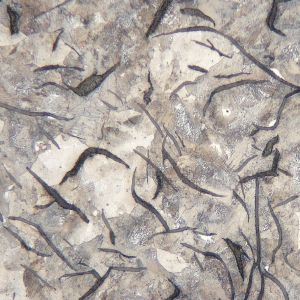
\includegraphics[scale=0.5]{pics/lamellengraphit}}
		\caption{Lamellengraphit (GJL)}
	\end{subfigure}\hfill
	\begin{subfigure}{0.32\textwidth}
		\centering
		\boxed{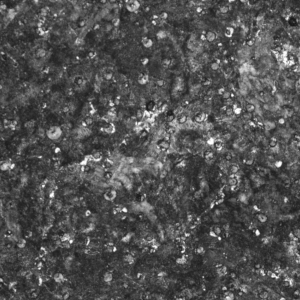
\includegraphics[scale=0.5]{pics/kugelgraphit}}
		\caption{Kugelgraphit (GJS)}
	\end{subfigure}\hfill
	\begin{subfigure}{0.32\textwidth}
		\centering
		\boxed{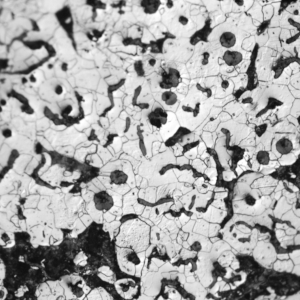
\includegraphics[scale=0.5]{pics/vermiculargraphit}}
		\caption{Vermiculargraphit (GJV)}
	\end{subfigure}
	\caption{Typen von Gusseisen nach Art der Graphitpartikelausbildung \cite{GiessereiLex2021}}
	\label{fig:GraphitTypes}
\end{figure}

\noindent Dabei unterscheiden sich die Gusseisenwerkstoffe nicht nur hinsichtlich der Form und Struktur ihrer Graphiteinlagerungen, sondern vor allem auch in Bezug auf die damit unmittelbar in Zusammenhang stehenden mechanischen Eigenschaften, wie bspw. Zug- und Druckfestigkeit, Bruchsicherheit oder plastische Verformbarkeit. Das bedeutet, dass bei Kräfteeinwirkung je nach Art unterschiedliche Spannungskonzentrationen in den Graphiteinschlüssen entstehen und der jeweilige Werkstoff sich somit mehr oder weniger für bestimmte Verwendungszwecke eignet.
\\\\
\noindent Die wichtigsten Abnehmer für von Gusswerkstoffen sind der Straßenfahrzeugbau mit fast 60~\% sowie der Maschinenbau mit 25 bis 30~\% der gesamten Gusslieferungen \cite{BDGuss01}.




\chapter{Grundlagen}
\label{ch:Grundlagen}

\section{Graphitklassifizierung}
\label{sec:Graphitklassifizierung}

\subsection{Lamellengraphit}
\label{subsec:Lamellengraphit}

\subsection{Mechanische Eigenschaften von Lamellengraphit}
\label{subsec:MechanischeEigenschaften}

\subsection{Einteilung von Gusseisen mit Lamellengraphit entsprechend den mechanischen Eigenschaften}
\label{subsec:EinteilungLamellengraphit}

\section{Grundlagen der Bildverarbeitung}
\label{GrundlagenBildverarbeitung}

\subsection{Bildrepräsentation und Farbräume}
\label{Bildrep}

\subsection{Bildskalierung und Interpolationsverfahren}
\label{subsec:SkalierungUndInterpolation}

Unter Bildskalierung versteht man die Vergrößerung bzw. Verkleinerung von Bildern. Es handelt sich dabei um ein Standardverfahren, welches sowohl im Grafik- und Fotobereich als auch in der digitalen Bildverarbeitung sehr häufig zum Einsatz kommt und von Bildverarbeitungsprogrammen standardmäßig angeboten wird. Da die algorithmische Funktionsweise einer Bildskalierung für das Verständnis der in dieser Arbeit zu lösenden Problemstellung (siehe auch Kapitel \ref{sec:Problemstellung} auf Seite \pageref{sec:Problemstellung}) von zentraler Bedeutung ist, wird diese nun hier genauer Untersucht und beschrieben.
\\\\
Das grundsätzliche Problem bei der Skalierung von Bildern, soll durch Abbildung \ref{fig:ScalingProblem} verdeutlicht werden. Zu sehen ist links ein Bild mit ($4\times 4$) Pixeln (orange) und rechts das durch Skalierung erzeugte Bild. Die neue Position eines beliebigen Originalpixels im neu erzeugten (skalierten) Bild ergibt sich durch Multiplikation der ursprünglichen Position mit dem Skalierungsfaktor ($\lambda$).
\begin{figure}[H]
	\centering
		\begin{tikzpicture}[x=0.75pt,y=0.75pt,yscale=-1,xscale=1, scale=0.9, every node/.style={scale=0.9}]
			%uncomment if require: \path (0,300); %set diagram left start at 0, 	and has height of 300
			
			%Shape: Rectangle [id:dp33493272980948086] 
			\draw  [color={rgb, 255:red, 255; green, 255; blue, 255 }  ,draw 	opacity=1 ][fill={rgb, 255:red, 0; green, 0; blue,  }  ,fill opacity=1 ] (240,53.85) -- (400,53.85) -- (400,213.85) -- (240,213.85) -- cycle ;
			%Shape: Grid [id:dp5166847032058127] 
			\draw  [draw opacity=0][fill={rgb, 255:red, 245; green, 166; blue, 35 }  ,fill opacity=1 ][line width=1.5]  (35.38,93.85) -- (116.38,93.85) -- (116.38,174.85) -- (35.38,174.85) -- cycle ; \draw  [line width=1.5]  (35.38,93.85) -- (35.38,174.85)(55.38,93.85) -- (55.38,174.85)(75.38,93.85) -- (75.38,174.85)(95.38,93.85) -- (95.38,174.85)(115.38,93.85) -- 	(115.38,174.85) ; \draw  [line width=1.5]  (35.38,93.85) -- (116.38,93.85)(35.38,113.85) -- (116.38,113.85)(35.38,133.85) -- (116.38,133.85)(35.38,153.85) -- (116.38,153.85)(35.38,173.85) -- (116.38,173.85) ; \draw  [line width=1.5]   ;
			%Right Arrow [id:dp7963578241503881] 
			\draw  [line width=1.5]  (139.38,123.71) -- (172.98,123.71) -- 	(172.98,116) -- (195.38,131.43) -- (172.98,146.85) -- (172.98,139.14) -- (139.38,139.14) -- cycle ;
			%Shape: Grid [id:dp813346916234577] 
			\draw  [draw opacity=0][line width=1.5]  (240,53.85) -- 	(400.38,53.85) -- (400.38,214.85) -- (240,214.85) -- cycle ; \draw  [color={rgb, 255:red, 0; green, 0; blue, 0 }  ,draw opacity=1 ][line width=1.5]  (240,53.85) -- (240,214.85)(260,53.85) -- (260,214.85)(280,53.85) -- (280,214.85)(300,53.85) -- (300,214.85)(320,53.85) -- (320,214.85)(340,53.85) -- (340,214.85)(360,53.85) -- (360,214.85)(380,53.85) -- (380,214.85)(400,53.85) -- (400,214.85) ; \draw  [color={rgb, 255:red, 0; green, 0; blue, 0 }  ,draw opacity=1 ][line width=1.5]  (240,53.85) -- (400.38,53.85)(240,73.85) -- (400.38,73.85)(240,93.85) -- (400.38,93.85)(240,113.85) -- (400.38,113.85)(240,133.85) -- (400.38,133.85)(240,153.85) -- (400.38,153.85)(240,173.85) -- (400.38,173.85)(240,193.85) -- (400.38,193.85)(240,213.85) -- (400.38,213.85) ; \draw  [color={rgb, 255:red, 0; green, 0; blue, 0 }  ,draw opacity=1 ][line width=1.5]   ;
			%Shape: Rectangle [id:dp7852221432702648] 
			\draw  [fill={rgb, 255:red, 245; green, 166; blue, 35 }  ,fill 	opacity=1 ][line width=1.5]  (240,53.85) -- (260,53.85) -- (260,73.85) -- (240,73.85) -- cycle ;
			%Shape: Rectangle [id:dp316493263782738] 
			\draw  [fill={rgb, 255:red, 245; green, 166; blue, 35 }  ,fill 	opacity=1 ][line width=1.5]  (360,53.85) -- (380,53.85) -- (380,73.85) -- (360,73.85) -- cycle ;
			%Shape: Rectangle [id:dp9150879931583693] 
			\draw  [fill={rgb, 255:red, 245; green, 166; blue, 35 }  ,fill 	opacity=1 ][line width=1.5]  (280,53.85) -- (300,53.85) -- (300,73.85) -- (280,73.85) -- cycle ;
			%Shape: Rectangle [id:dp21254213121480348] 
			\draw  [fill={rgb, 255:red, 245; green, 166; blue, 35 }  ,fill 	opacity=1 ][line width=1.5]  (320,53.85) -- (340,53.85) -- (340,73.85) -- (320,73.85) -- cycle ;
			%Shape: Rectangle [id:dp9138059724854111] 
			\draw  [fill={rgb, 255:red, 245; green, 166; blue, 35 }  ,fill 	opacity=1 ][line width=1.5]  (240,93.85) -- (260,93.85) -- (260,113.85) -- (240,113.85) -- cycle ;
			%Shape: Rectangle [id:dp8385734790799879] 
			\draw  [fill={rgb, 255:red, 245; green, 166; blue, 35 }  ,fill 	opacity=1 ][line width=1.5]  (360,93.85) -- (380,93.85) -- (380,113.85) -- (360,113.85) -- cycle ;
			%Shape: Rectangle [id:dp0266783762407925] 
			\draw  [fill={rgb, 255:red, 245; green, 166; blue, 35 }  ,fill 	opacity=1 ][line width=1.5]  (280,93.85) -- (300,93.85) -- (300,113.85) -- (280,113.85) -- cycle ;
			%Shape: Rectangle [id:dp8765432738424186] 
			\draw  [fill={rgb, 255:red, 245; green, 166; blue, 35 }  ,fill 	opacity=1 ][line width=1.5]  (320,93.85) -- (340,93.85) -- (340,113.85) -- (320,113.85) -- cycle ;
			%Shape: Rectangle [id:dp3683961028684497] 
			\draw  [fill={rgb, 255:red, 245; green, 166; blue, 35 }  ,fill 	opacity=1 ][line width=1.5]  (240,133.85) -- (260,133.85) -- (260,153.85) -- (240,153.85) -- cycle ;
			%Shape: Rectangle [id:dp17023134792901806] 
			\draw  [fill={rgb, 255:red, 245; green, 166; blue, 35 }  ,fill 	opacity=1 ][line width=1.5]  (360,133.85) -- (380,133.85) -- (380,153.85) -- (360,153.85) -- cycle ;
			%Shape: Rectangle [id:dp30885139351862023] 
			\draw  [fill={rgb, 255:red, 245; green, 166; blue, 35 }  ,fill 	opacity=1 ][line width=1.5]  (280,133.85) -- (300,133.85) -- (300,153.85) -- (280,153.85) -- cycle ;
			%Shape: Rectangle [id:dp2063497064425942] 
			\draw  [fill={rgb, 255:red, 245; green, 166; blue, 35 }  ,fill 	opacity=1 ][line width=1.5]  (320,133.85) -- (340,133.85) -- (340,153.85) -- (320,153.85) -- cycle ;
			%Shape: Rectangle [id:dp7893916008859733] 
			\draw  [fill={rgb, 255:red, 245; green, 166; blue, 35 }  ,fill 	opacity=1 ][line width=1.5]  (240,173.85) -- (260,173.85) -- (260,193.85) -- (240,193.85) -- cycle ;
			%Shape: Rectangle [id:dp03560102427440881] 
			\draw  [fill={rgb, 255:red, 245; green, 166; blue, 35 }  ,fill 	opacity=1 ][line width=1.5]  (360,173.85) -- (380,173.85) -- (380,193.85) -- (360,193.85) -- cycle ;
			%Shape: Rectangle [id:dp5475282364153556] 
			\draw  [fill={rgb, 255:red, 245; green, 166; blue, 35 }  ,fill 	opacity=1 ][line width=1.5]  (280,173.85) -- (300,173.85) -- (300,193.85) -- (280,193.85) -- cycle ;
			%Shape: Rectangle [id:dp34756519033919797] 
			\draw  [fill={rgb, 255:red, 245; green, 166; blue, 35 }  ,fill 	opacity=1 ][line width=1.5]  (320,173.85) -- (340,173.85) -- (340,193.85) -- (320,193.85) -- cycle ;
			%Straight Lines [id:da27131202915211117] 
			\draw    (17.38,69.85) -- (143.38,69.85) ;
			\draw [shift={(145.38,69.85)}, rotate = 180] [color={rgb, 255:red, 	0; green, 0; blue, 0 }  ][line width=0.75]    (10.93,-3.29) .. controls (6.95,-1.4) and (3.31,-0.3) .. (0,0) .. controls (3.31,0.3) and (6.95,1.4) .. (10.93,3.29)   ;
			%Straight Lines [id:da0003577742395167727] 
			\draw    (17.38,69.85) -- (17.38,198.85) ;
			\draw [shift={(17.38,200.85)}, rotate = 270] [color={rgb, 255:red, 	0; green, 0; blue, 0 }  ][line width=0.75]    (10.93,-3.29) .. controls (6.95,-1.4) and (3.31,-0.3) .. (0,0) .. controls (3.31,0.3) and (6.95,1.4) .. (10.93,3.29)   ;
			%Straight Lines [id:da8167500493181958] 
			\draw    (218.38,26.85) -- (447.38,26.85) ;
			\draw [shift={(449.38,26.85)}, rotate = 180] [color={rgb, 255:red, 	0; green, 0; blue, 0 }  ][line width=0.75]    (10.93,-3.29) .. controls (6.95,-1.4) and (3.31,-0.3) .. (0,0) .. controls (3.31,0.3) and (6.95,1.4) .. (10.93,3.29)   ;
			%Straight Lines [id:da5628538454694642] 
			\draw    (218.38,26.85) -- (218.38,244.85) ;
			\draw [shift={(218.38,246.85)}, rotate = 270] [color={rgb, 255:red, 	0; green, 0; blue, 0 }  ][line width=0.75]    (10.93,-3.29) .. controls (6.95,-1.4) and (3.31,-0.3) .. (0,0) .. controls (3.31,0.3) and (6.95,1.4) .. (10.93,3.29)   ;
			
			% Text Node
			\draw (142.38,125.71) node [anchor=north west][inner sep=0.75pt]  	[font=\normalsize] [align=left] {$\displaystyle \lambda $\textbf{ = 2}};
			% Text Node
			\draw (49,231) node [anchor=north west][inner sep=0.75pt]   [align=left] {\textcolor[rgb]{0,0,0}{$\displaystyle \lambda 	$}\textcolor[rgb]{0,0,0}{\textbf{: Skalierungsfaktor}}};
			% Text Node
			\draw (23,96) node [anchor=north west][inner sep=0.75pt]   	[align=left] {0};
			% Text Node
			\draw (23,116) node [anchor=north west][inner sep=0.75pt]   	[align=left] {1};
			% Text Node
			\draw (23,136) node [anchor=north west][inner sep=0.75pt]   	[align=left] {2};
			% Text Node
			\draw (23,157) node [anchor=north west][inner sep=0.75pt]   	[align=left] {3};
			% Text Node
			\draw (40,79) node [anchor=north west][inner sep=0.75pt]   	[align=left] {0};
			% Text Node
			\draw (60,79) node [anchor=north west][inner sep=0.75pt]   	[align=left] {1};
			% Text Node
			\draw (80,79) node [anchor=north west][inner sep=0.75pt]   	[align=left] {2};
			% Text Node
			\draw (101,79) node [anchor=north west][inner sep=0.75pt]   	[align=left] {3};
			% Text Node
			\draw (150,66) node [anchor=north west][inner sep=0.75pt]   	[align=left] {x};
			% Text Node
			\draw (13,206) node [anchor=north west][inner sep=0.75pt]   	[align=left] {y};
			% Text Node
			\draw (244,38) node [anchor=north west][inner sep=0.75pt]   	[align=left] {0};
			% Text Node
			\draw (264,38) node [anchor=north west][inner sep=0.75pt]   	[align=left] {1};
			% Text Node
			\draw (284,38) node [anchor=north west][inner sep=0.75pt]   	[align=left] {2};
			% Text Node
			\draw (305,38) node [anchor=north west][inner sep=0.75pt]   	[align=left] {3};
			% Text Node
			\draw (325,38) node [anchor=north west][inner sep=0.75pt]   	[align=left] {4};
			% Text Node
			\draw (345,38) node [anchor=north west][inner sep=0.75pt]   	[align=left] {5};
			% Text Node
			\draw (365,38) node [anchor=north west][inner sep=0.75pt]   	[align=left] {6};
			% Text Node
			\draw (384,38) node [anchor=north west][inner sep=0.75pt]   	[align=left] {7};
			% Text Node
			\draw (227,56) node [anchor=north west][inner sep=0.75pt]   	[align=left] {0};
			% Text Node
			\draw (227,76) node [anchor=north west][inner sep=0.75pt]   	[align=left] {1};
			% Text Node
			\draw (227,96) node [anchor=north west][inner sep=0.75pt]   	[align=left] {2};
			% Text Node
			\draw (227,117) node [anchor=north west][inner sep=0.75pt]   	[align=left] {3};
			% Text Node
			\draw (227,137) node [anchor=north west][inner sep=0.75pt]   	[align=left] {4};
			% Text Node
			\draw (227,157) node [anchor=north west][inner sep=0.75pt]   	[align=left] {5};
			% Text Node
			\draw (227,176) node [anchor=north west][inner sep=0.75pt]   	[align=left] {6};
			% Text Node
			\draw (227,197) node [anchor=north west][inner sep=0.75pt]   	[align=left] {7};
			% Text Node
			\draw (455,24) node [anchor=north west][inner sep=0.75pt]   	[align=left] {x};
			% Text Node
			\draw (214,252) node [anchor=north west][inner sep=0.75pt]   	[align=left] {y};
		\end{tikzpicture}
	\caption{Darstellung der Notwendigkeit von\\ Interpolationsverfahren bei der Bildskalierung}
	\label{fig:ScalingProblem}
\end{figure}

\noindent Genauer ausgedrückt handelt es sich bei den Lücken um undefinierte Pixel, da sich die Pixelmenge proportional zum Skalierungsfaktor ebenfalls verändert. Bei Skalierungsfaktoren kleiner 1 verhält es sich genau umgekehrt und die Anzahl der Pixel im Ergebnisbild verringert sich entsprechend.
\\\\
\noindent Zur Lösung dieses Problems wurden verschiedene Interpolationsalgorithmen entwickelt. Diese verfolgen alle das Ziel, die sich ergebende Differenz der Pixelanzahl auszugleichen und die Bildqualität dadurch möglichst gut zu erhalten. Dabei werden also die Farbwerte der grauen (undefinierten) Pixel aus den Farbwerten der umliegenden Pixel auf jeweils unterschiedliche Art approximiert. Es liegt jedoch auf der Hand, das ein solchen Verfahren die Details eines gegebenen Originalbildes nie 100\%-ig erhalten kann. So können zwar für viele praktische Anwendungsfälle im Grafik- oder Fotobereich sehr gute Ergebnisse erzielt werden, weil das menschliche Auge diese Abweichungen nicht erkennen kann. Allerdings erweist sich die Interpolation im Bereich der bildbasierten Materialstrukturanalyse als problematisch, da sich  die zu analysierenden Strukturen durch die Interpolation verändern und somit die Messergebnisse verfälscht werden. Während diese Problematik in Kapitel \ref{sec:Problemstellung} auf Seite \pageref{sec:Problemstellung} im Detail beschrieben wird konzentriert sich die nachfolgende Darstellung nun zunächst darauf darzustellen, wie die verschiedenen Algorithmen funktionieren und worin die Unterschiede liegen.
\\\\
\textbf{Bilineare Interpolation}\label{par:LinearInterpol}
\\\\
Bei der bilinearen Interpolation handelt es sich um ein sehr einfaches Verfahren, bei dem zur Bestimmung unbestimmter Pixel nach der Skalierung, deren Farbwerte (RGB) durch lineare Interpolation in X- und Y-Richtung berechnet werden. Als Beispiel dient folgende Situation, die in Abbildung \ref{fig:BilinearInterpolation1} dargestellt ist.

\begin{figure}[H]
	\centering
	\begin{tikzpicture}[x=0.75pt,y=0.75pt,yscale=-1,xscale=1, scale=1.2, every node/.style={scale=1.2}]
		%uncomment if require: \path (0,374); %set diagram left start at 0, and has height of 374
		
		%Shape: Grid [id:dp6031282918603735] 
		\draw  [draw opacity=0][line width=1.5]  (300.38,50.85) -- (481.38,50.85) -- (481.38,231.85) -- (300.38,231.85) -- cycle ; \draw  [color={rgb, 255:red, 0; green, 0; blue, 0 }  ,draw opacity=1 ][line width=1.5]  (300.38,50.85) -- (300.38,231.85)(330.38,50.85) -- (330.38,231.85)(360.38,50.85) -- (360.38,231.85)(390.38,50.85) -- (390.38,231.85)(420.38,50.85) -- (420.38,231.85)(450.38,50.85) -- (450.38,231.85)(480.38,50.85) -- (480.38,231.85) ; \draw  [color={rgb, 255:red, 0; green, 0; blue, 0 }  ,draw opacity=1 ][line width=1.5]  (300.38,50.85) -- (481.38,50.85)(300.38,80.85) -- (481.38,80.85)(300.38,110.85) -- (481.38,110.85)(300.38,140.85) -- (481.38,140.85)(300.38,170.85) -- (481.38,170.85)(300.38,200.85) -- (481.38,200.85)(300.38,230.85) -- (481.38,230.85) ; \draw  [color={rgb, 255:red, 0; green, 0; blue, 0 }  ,draw opacity=1 ][line width=1.5]   ;
		%Shape: Axis 2D [id:dp12421444962330219] 
		\draw  (283.56,4.16) -- (283.56,260.85)(506.38,29.83) -- (258.81,29.83) (288.56,253.85) -- (283.56,260.85) -- (278.56,253.85) (499.38,24.83) -- (506.38,29.83) -- (499.38,34.83)  ;
		%Shape: Axis 2D [id:dp5582126406856516] 
		\draw  (43.86,14.16) -- (43.86,166.85)(188.38,29.43) -- (27.81,29.43) (48.86,159.85) -- (43.86,166.85) -- (38.86,159.85) (181.38,24.43) -- (188.38,29.43) -- (181.38,34.43)  ;
		%Shape: Grid [id:dp6426300130896345] 
		\draw  [draw opacity=0][line width=2.25]  (62,51) -- (152.38,51) -- (152.38,141.85) -- (62,141.85) -- cycle ; \draw  [line width=2.25]  (62,51) -- (62,141.85)(92,51) -- (92,141.85)(122,51) -- (122,141.85)(152,51) -- (152,141.85) ; \draw  [line width=2.25]  (62,51) -- (152.38,51)(62,81) -- (152.38,81)(62,111) -- (152.38,111)(62,141) -- (152.38,141) ; \draw  [line width=2.25]   ;
		%Shape: Rectangle [id:dp13871600656081773] 
		\draw  [fill={rgb, 255:red, 245; green, 166; blue, 35 }  ,fill opacity=1 ][line width=1.5]  (92,51) -- (122,51) -- (122,81) -- (92,81) -- cycle ;
		%Shape: Rectangle [id:dp09914050619225745] 
		\draw  [fill={rgb, 255:red, 245; green, 166; blue, 35 }  ,fill opacity=1 ][line width=1.5]  (122,81) -- (152,81) -- (152,111) -- (122,111) -- cycle ;
		%Shape: Rectangle [id:dp7354425170625416] 
		\draw  [fill={rgb, 255:red, 245; green, 166; blue, 35 }  ,fill opacity=1 ][line width=1.5]  (122,111) -- (152,111) -- (152,141) -- (122,141) -- cycle ;
		%Shape: Rectangle [id:dp8022069903462297] 
		\draw  [fill={rgb, 255:red, 245; green, 166; blue, 35 }  ,fill opacity=1 ][line width=1.5]  (62,111) -- (92,111) -- (92,141) -- (62,141) -- cycle ;
		%Shape: Rectangle [id:dp5675136532554508] 
		\draw  [fill={rgb, 255:red, 245; green, 166; blue, 35 }  ,fill opacity=1 ][line width=1.5]  (92,111) -- (122,111) -- (122,141) -- (92,141) -- cycle ;
		%Shape: Rectangle [id:dp26546030668596743] 
		\draw  [fill={rgb, 255:red, 126; green, 211; blue, 33 }  ,fill opacity=1 ][line width=1.5]  (122,51) -- (152,51) -- (152,81) -- (122,81) -- cycle ;
		%Shape: Rectangle [id:dp31022250660119444] 
		\draw  [fill={rgb, 255:red, 126; green, 211; blue, 33 }  ,fill opacity=1 ][line width=1.5]  (92,81) -- (122,81) -- (122,111) -- (92,111) -- cycle ;
		%Shape: Rectangle [id:dp1632256531496281] 
		\draw  [fill={rgb, 255:red, 126; green, 211; blue, 33 }  ,fill opacity=1 ][line width=1.5]  (62,51) -- (92,51) -- (92,81) -- (62,81) -- cycle ;
		%Shape: Rectangle [id:dp36586491405776467] 
		\draw  [fill={rgb, 255:red, 126; green, 211; blue, 33 }  ,fill opacity=1 ][line width=1.5]  (62,81) -- (92,81) -- (92,111) -- (62,111) -- cycle ;
		%Shape: Rectangle [id:dp09483486001396602] 
		\draw  [fill={rgb, 255:red, 245; green, 166; blue, 35 }  ,fill opacity=1 ][line width=1.5]  (360.38,50.85) -- (390.38,50.85) -- (390.38,80.85) -- (360.38,80.85) -- cycle ;
		%Shape: Rectangle [id:dp8722790379045016] 
		\draw  [fill={rgb, 255:red, 245; green, 166; blue, 35 }  ,fill opacity=1 ][line width=1.5]  (420.38,110.85) -- (450.38,110.85) -- (450.38,140.85) -- (420.38,140.85) -- cycle ;
		%Shape: Rectangle [id:dp3090077325311579] 
		\draw  [fill={rgb, 255:red, 245; green, 166; blue, 35 }  ,fill opacity=1 ][line width=1.5]  (420.38,170.85) -- (450.38,170.85) -- (450.38,200.85) -- (420.38,200.85) -- cycle ;
		%Shape: Rectangle [id:dp39265423932322685] 
		\draw  [fill={rgb, 255:red, 245; green, 166; blue, 35 }  ,fill opacity=1 ][line width=1.5]  (300.38,170.85) -- (330.38,170.85) -- (330.38,200.85) -- (300.38,200.85) -- cycle ;
		%Shape: Rectangle [id:dp309527828572457] 
		\draw  [fill={rgb, 255:red, 245; green, 166; blue, 35 }  ,fill opacity=1 ][line width=1.5]  (360.38,170.85) -- (390.38,170.85) -- (390.38,200.85) -- (360.38,200.85) -- cycle ;
		%Shape: Rectangle [id:dp43382954399056994] 
		\draw  [fill={rgb, 255:red, 126; green, 211; blue, 33 }  ,fill opacity=1 ][line width=1.5]  (420.38,50.85) -- (450.38,50.85) -- (450.38,80.85) -- (420.38,80.85) -- cycle ;
		%Shape: Rectangle [id:dp5113204315472576] 
		\draw  [fill={rgb, 255:red, 126; green, 211; blue, 33 }  ,fill opacity=1 ][line width=1.5]  (360.38,110.85) -- (390.38,110.85) -- (390.38,140.85) -- (360.38,140.85) -- cycle ;
		%Shape: Rectangle [id:dp06279947117329954] 
		\draw  [fill={rgb, 255:red, 126; green, 211; blue, 33 }  ,fill opacity=1 ][line width=1.5]  (300.38,50.85) -- (330.38,50.85) -- (330.38,80.85) -- (300.38,80.85) -- cycle ;
		%Shape: Rectangle [id:dp7495389450561212] 
		\draw  [fill={rgb, 255:red, 126; green, 211; blue, 33 }  ,fill opacity=1 ][line width=1.5]  (300.38,110.85) -- (330.38,110.85) -- (330.38,140.85) -- (300.38,140.85) -- cycle ;
		%Shape: Rectangle [id:dp3179677452191165] 
		\draw  [color={rgb, 255:red, 0; green, 0; blue, 0 }  ,draw opacity=1 ][fill={rgb, 255:red, 185; green, 188; blue, 34 }  ,fill opacity=1 ][line width=1.5]  (330.38,50.85) -- (360.38,50.85) -- (360.38,80.85) -- (330.38,80.85) -- cycle ;
		%Shape: Rectangle [id:dp02520564590269525] 
		\draw  [color={rgb, 255:red, 0; green, 0; blue, 0 }  ,draw opacity=1 ][fill={rgb, 255:red, 185; green, 188; blue, 34 }  ,fill opacity=1 ][line width=1.5]  (390.38,50.85) -- (420.38,50.85) -- (420.38,80.85) -- (390.38,80.85) -- cycle ;
		%Shape: Rectangle [id:dp41456521365377197] 
		\draw  [color={rgb, 255:red, 0; green, 0; blue, 0 }  ,draw opacity=1 ][fill={rgb, 255:red, 185; green, 188; blue, 34 }  ,fill opacity=1 ][line width=1.5]  (360.38,80.85) -- (390.38,80.85) -- (390.38,110.85) -- (360.38,110.85) -- cycle ;
		%Shape: Rectangle [id:dp7715421317421746] 
		\draw  [color={rgb, 255:red, 0; green, 0; blue, 0 }  ,draw opacity=1 ][fill={rgb, 255:red, 185; green, 188; blue, 34 }  ,fill opacity=1 ][line width=1.5]  (420.38,80.85) -- (450.38,80.85) -- (450.38,110.85) -- (420.38,110.85) -- cycle ;
		%Shape: Rectangle [id:dp6537803831672764] 
		\draw  [color={rgb, 255:red, 0; green, 0; blue, 0 }  ,draw opacity=1 ][fill={rgb, 255:red, 185; green, 188; blue, 34 }  ,fill opacity=1 ][line width=1.5]  (390.38,110.85) -- (420.38,110.85) -- (420.38,140.85) -- (390.38,140.85) -- cycle ;
		%Shape: Rectangle [id:dp694492919060651] 
		\draw  [color={rgb, 255:red, 0; green, 0; blue, 0 }  ,draw opacity=1 ][fill={rgb, 255:red, 185; green, 188; blue, 34 }  ,fill opacity=1 ][line width=1.5]  (390.38,80.85) -- (420.38,80.85) -- (420.38,110.85) -- (390.38,110.85) -- cycle ;
		%Shape: Rectangle [id:dp8749183811880095] 
		\draw  [color={rgb, 255:red, 0; green, 0; blue, 0 }  ,draw opacity=1 ][fill={rgb, 255:red, 185; green, 188; blue, 34 }  ,fill opacity=1 ][line width=1.5]  (300.38,140.85) -- (330.38,140.85) -- (330.38,170.85) -- (300.38,170.85) -- cycle ;
		%Shape: Rectangle [id:dp15019771324119735] 
		\draw  [color={rgb, 255:red, 0; green, 0; blue, 0 }  ,draw opacity=1 ][fill={rgb, 255:red, 185; green, 188; blue, 34 }  ,fill opacity=1 ][line width=1.5]  (360.38,140.85) -- (390.38,140.85) -- (390.38,170.85) -- (360.38,170.85) -- cycle ;
		%Shape: Rectangle [id:dp8886413553682353] 
		\draw  [color={rgb, 255:red, 0; green, 0; blue, 0 }  ,draw opacity=1 ][fill={rgb, 255:red, 185; green, 188; blue, 34 }  ,fill opacity=1 ][line width=1.5]  (330.38,140.85) -- (360.38,140.85) -- (360.38,170.85) -- (330.38,170.85) -- cycle ;
		%Shape: Rectangle [id:dp18893376895528624] 
		\draw  [fill={rgb, 255:red, 245; green, 166; blue, 35 }  ,fill opacity=1 ][line width=1.5]  (420.38,140.85) -- (450.38,140.85) -- (450.38,170.85) -- (420.38,170.85) -- cycle ;
		%Shape: Rectangle [id:dp8401086030387102] 
		\draw  [fill={rgb, 255:red, 245; green, 166; blue, 35 }  ,fill opacity=1 ][line width=1.5]  (390.38,170.85) -- (420.38,170.85) -- (420.38,200.85) -- (390.38,200.85) -- cycle ;
		%Shape: Rectangle [id:dp5023664828243175] 
		\draw  [fill={rgb, 255:red, 245; green, 166; blue, 35 }  ,fill opacity=1 ][line width=1.5]  (330.38,170.85) -- (360.38,170.85) -- (360.38,200.85) -- (330.38,200.85) -- cycle ;
		%Shape: Rectangle [id:dp4926347479761316] 
		\draw  [fill={rgb, 255:red, 126; green, 211; blue, 33 }  ,fill opacity=1 ][line width=1.5]  (300.38,80.85) -- (330.38,80.85) -- (330.38,110.85) -- (300.38,110.85) -- cycle ;
		%Shape: Rectangle [id:dp03314094385373201] 
		\draw  [fill={rgb, 255:red, 126; green, 211; blue, 33 }  ,fill opacity=1 ][line width=1.5]  (330.38,110.85) -- (360.38,110.85) -- (360.38,140.85) -- (330.38,140.85) -- cycle ;
		%Shape: Rectangle [id:dp31700461022402926] 
		\draw  [color={rgb, 255:red, 0; green, 0; blue, 0 }  ,draw opacity=1 ][fill={rgb, 255:red, 155; green, 199; blue, 33 }  ,fill opacity=1 ][line width=1.5]  (330.38,80.85) -- (360.38,80.85) -- (360.38,110.85) -- (330.38,110.85) -- cycle ;
		%Shape: Rectangle [id:dp17649729390737434] 
		\draw  [color={rgb, 255:red, 0; green, 0; blue, 0 }  ,draw opacity=1 ][fill={rgb, 255:red, 215; green, 177; blue, 34 }  ,fill opacity=1 ][line width=1.5]  (390.38,140.85) -- (420.38,140.85) -- (420.38,170.85) -- (390.38,170.85) -- cycle ;
		%Right Arrow [id:dp33270781304422914] 
		\draw  [line width=1.5]  (185,86) -- (227,86) -- (227,76) -- (255,96) -- (227,116) -- (227,106) -- (185,106) -- cycle ;
		%Shape: Rectangle [id:dp24983247014857224] 
		\draw  [fill={rgb, 255:red, 126; green, 211; blue, 33 }  ,fill opacity=1 ][line width=1.5]  (450.38,50.85) -- (480.38,50.85) -- (480.38,80.85) -- (450.38,80.85) -- cycle ;
		%Shape: Rectangle [id:dp35849526261121356] 
		\draw  [fill={rgb, 255:red, 245; green, 166; blue, 35 }  ,fill opacity=1 ][line width=1.5]  (450.38,110.85) -- (480.38,110.85) -- (480.38,140.85) -- (450.38,140.85) -- cycle ;
		%Shape: Rectangle [id:dp1351111821765797] 
		\draw  [fill={rgb, 255:red, 245; green, 166; blue, 35 }  ,fill opacity=1 ][line width=1.5]  (450.38,170.85) -- (480.38,170.85) -- (480.38,200.85) -- (450.38,200.85) -- cycle ;
		%Shape: Rectangle [id:dp5617796085771564] 
		\draw  [color={rgb, 255:red, 0; green, 0; blue, 0 }  ,draw opacity=1 ][fill={rgb, 255:red, 185; green, 188; blue, 34 }  ,fill opacity=1 ][line width=1.5]  (450.38,80.85) -- (480.38,80.85) -- (480.38,110.85) -- (450.38,110.85) -- cycle ;
		%Shape: Rectangle [id:dp6849626334604124] 
		\draw  [fill={rgb, 255:red, 245; green, 166; blue, 35 }  ,fill opacity=1 ][line width=1.5]  (450.38,140.85) -- (480.38,140.85) -- (480.38,170.85) -- (450.38,170.85) -- cycle ;
		%Shape: Rectangle [id:dp4423643524339804] 
		\draw  [fill={rgb, 255:red, 245; green, 166; blue, 35 }  ,fill opacity=1 ][line width=1.5]  (420.38,200.85) -- (450.38,200.85) -- (450.38,230.85) -- (420.38,230.85) -- cycle ;
		%Shape: Rectangle [id:dp9844308475991588] 
		\draw  [fill={rgb, 255:red, 245; green, 166; blue, 35 }  ,fill opacity=1 ][line width=1.5]  (300.38,200.85) -- (330.38,200.85) -- (330.38,230.85) -- (300.38,230.85) -- cycle ;
		%Shape: Rectangle [id:dp19330105393002595] 
		\draw  [fill={rgb, 255:red, 245; green, 166; blue, 35 }  ,fill opacity=1 ][line width=1.5]  (360.38,200.85) -- (390.38,200.85) -- (390.38,230.85) -- (360.38,230.85) -- cycle ;
		%Shape: Rectangle [id:dp719400766119336] 
		\draw  [fill={rgb, 255:red, 245; green, 166; blue, 35 }  ,fill opacity=1 ][line width=1.5]  (390.38,200.85) -- (420.38,200.85) -- (420.38,230.85) -- (390.38,230.85) -- cycle ;
		%Shape: Rectangle [id:dp3277584194542974] 
		\draw  [fill={rgb, 255:red, 245; green, 166; blue, 35 }  ,fill opacity=1 ][line width=1.5]  (330.38,200.85) -- (360.38,200.85) -- (360.38,230.85) -- (330.38,230.85) -- cycle ;
		%Shape: Rectangle [id:dp5673130666239078] 
		\draw  [fill={rgb, 255:red, 245; green, 166; blue, 35 }  ,fill opacity=1 ][line width=1.5]  (450.38,200.85) -- (480.38,200.85) -- (480.38,230.85) -- (450.38,230.85) -- cycle ;
		%Left Right Arrow [id:dp10603987349893162] 
		\draw  [color={rgb, 255:red, 255; green, 255; blue, 255 }  ,draw opacity=1 ] (334.19,65.85) -- (339.79,58.43) -- (339.79,62.14) -- (350.98,62.14) -- (350.98,58.43) -- (356.57,65.85) -- (350.98,73.28) -- (350.98,69.56) -- (339.79,69.56) -- (339.79,73.28) -- cycle ;
		%Left Right Arrow [id:dp4851771954641114] 
		\draw  [color={rgb, 255:red, 255; green, 255; blue, 255 }  ,draw opacity=1 ] (394.19,65.85) -- (399.79,58.43) -- (399.79,62.14) -- (410.98,62.14) -- (410.98,58.43) -- (416.57,65.85) -- (410.98,73.28) -- (410.98,69.56) -- (399.79,69.56) -- (399.79,73.28) -- cycle ;
		%Left Right Arrow [id:dp46535515779583203] 
		\draw  [color={rgb, 255:red, 255; green, 255; blue, 255 }  ,draw opacity=1 ] (334.19,185.85) -- (339.79,178.43) -- (339.79,182.14) -- (350.98,182.14) -- (350.98,178.43) -- (356.57,185.85) -- (350.98,193.28) -- (350.98,189.56) -- (339.79,189.56) -- (339.79,193.28) -- cycle ;
		%Left Right Arrow [id:dp0388460015786245] 
		\draw  [color={rgb, 255:red, 255; green, 255; blue, 255 }  ,draw opacity=1 ] (394.19,185.85) -- (399.79,178.43) -- (399.79,182.14) -- (410.98,182.14) -- (410.98,178.43) -- (416.57,185.85) -- (410.98,193.28) -- (410.98,189.56) -- (399.79,189.56) -- (399.79,193.28) -- cycle ;
		%Left Right Arrow [id:dp7225211430319548] 
		\draw  [color={rgb, 255:red, 255; green, 255; blue, 255 }  ,draw opacity=1 ] (334.19,125.85) -- (339.79,118.43) -- (339.79,122.14) -- (350.98,122.14) -- (350.98,118.43) -- (356.57,125.85) -- (350.98,133.28) -- (350.98,129.56) -- (339.79,129.56) -- (339.79,133.28) -- cycle ;
		%Left Right Arrow [id:dp4516242307309136] 
		\draw  [color={rgb, 255:red, 255; green, 255; blue, 255 }  ,draw opacity=1 ] (394.19,125.85) -- (399.79,118.43) -- (399.79,122.14) -- (410.98,122.14) -- (410.98,118.43) -- (416.57,125.85) -- (410.98,133.28) -- (410.98,129.56) -- (399.79,129.56) -- (399.79,133.28) -- cycle ;
		%Left Right Arrow [id:dp2240592597082971] 
		\draw  [color={rgb, 255:red, 255; green, 255; blue, 255 }  ,draw opacity=1 ] (315.4,84.66) -- (322.82,90.26) -- (319.1,90.26) -- (319.09,101.45) -- (322.8,101.45) -- (315.37,107.04) -- (307.95,101.44) -- (311.66,101.44) -- (311.68,90.25) -- (307.97,90.25) -- cycle ;
		%Left Right Arrow [id:dp526728801760665] 
		\draw  [color={rgb, 255:red, 255; green, 255; blue, 255 }  ,draw opacity=1 ] (315.4,144.66) -- (322.82,150.26) -- (319.1,150.26) -- (319.09,161.45) -- (322.8,161.45) -- (315.37,167.04) -- (307.95,161.44) -- (311.66,161.44) -- (311.68,150.25) -- (307.97,150.25) -- cycle ;
		%Left Right Arrow [id:dp5265171418673112] 
		\draw  [color={rgb, 255:red, 255; green, 255; blue, 255 }  ,draw opacity=1 ] (435.4,84.66) -- (442.82,90.26) -- (439.1,90.26) -- (439.09,101.45) -- (442.8,101.45) -- (435.37,107.04) -- (427.95,101.44) -- (431.66,101.44) -- (431.68,90.25) -- (427.97,90.25) -- cycle ;
		%Left Right Arrow [id:dp30991370393310413] 
		\draw  [color={rgb, 255:red, 255; green, 255; blue, 255 }  ,draw opacity=1 ] (435.4,144.66) -- (442.82,150.26) -- (439.1,150.26) -- (439.09,161.45) -- (442.8,161.45) -- (435.37,167.04) -- (427.95,161.44) -- (431.66,161.44) -- (431.68,150.25) -- (427.97,150.25) -- cycle ;
		%Left Right Arrow [id:dp38972009417085385] 
		\draw  [color={rgb, 255:red, 255; green, 255; blue, 255 }  ,draw opacity=1 ] (374.4,84.66) -- (381.82,90.26) -- (378.1,90.26) -- (378.09,101.45) -- (381.8,101.45) -- (374.37,107.04) -- (366.95,101.44) -- (370.66,101.44) -- (370.68,90.25) -- (366.97,90.25) -- cycle ;
		%Left Right Arrow [id:dp7707043216642973] 
		\draw  [color={rgb, 255:red, 255; green, 255; blue, 255 }  ,draw opacity=1 ] (375.4,144.66) -- (382.82,150.26) -- (379.1,150.26) -- (379.09,161.45) -- (382.8,161.45) -- (375.37,167.04) -- (367.95,161.44) -- (371.66,161.44) -- (371.68,150.25) -- (367.97,150.25) -- cycle ;

		
		% Text Node
		\draw (262,156.99) node [anchor=north west][inner sep=0.75pt]  [font=\normalsize,rotate=-270.08] [align=left] {$\displaystyle \lambda \cdot \ y$};
		% Text Node
		\draw (372.56,11) node [anchor=north west][inner sep=0.75pt]  [font=\normalsize,rotate=-359.4] [align=left] {\textcolor[rgb]{0,0,0}{$\displaystyle \lambda \cdot \ x$}};
		% Text Node
		\draw (309,35) node [anchor=north west][inner sep=0.75pt]   [align=left] {0};
		% Text Node
		\draw (340,35) node [anchor=north west][inner sep=0.75pt]   [align=left] {1};
		% Text Node
		\draw (371,35) node [anchor=north west][inner sep=0.75pt]   [align=left] {2};
		% Text Node
		\draw (398,35) node [anchor=north west][inner sep=0.75pt]   [align=left] {3};
		% Text Node
		\draw (431,35) node [anchor=north west][inner sep=0.75pt]   [align=left] {4};
		% Text Node
		\draw (288,58) node [anchor=north west][inner sep=0.75pt]   [align=left] {0};
		% Text Node
		\draw (288,89) node [anchor=north west][inner sep=0.75pt]   [align=left] {1};
		% Text Node
		\draw (288,119) node [anchor=north west][inner sep=0.75pt]   [align=left] {2};
		% Text Node
		\draw (288,148) node [anchor=north west][inner sep=0.75pt]   [align=left] {3};
		% Text Node
		\draw (288,179) node [anchor=north west][inner sep=0.75pt]   [align=left] {4};
		% Text Node
		\draw (510,25.5) node [anchor=north west][inner sep=0.75pt]   [align=left] {x};
		% Text Node
		\draw (40,170) node [anchor=north west][inner sep=0.75pt]   [align=left] {y};
		% Text Node
		\draw (71,35) node [anchor=north west][inner sep=0.75pt]   [align=left] {0};
		% Text Node
		\draw (102,35) node [anchor=north west][inner sep=0.75pt]   [align=left] {1};
		% Text Node
		\draw (133,35) node [anchor=north west][inner sep=0.75pt]   [align=left] {2};
		% Text Node
		\draw (49,58) node [anchor=north west][inner sep=0.75pt]   [align=left] {0};
		% Text Node
		\draw (49,89) node [anchor=north west][inner sep=0.75pt]   [align=left] {1};
		% Text Node
		\draw (49,119) node [anchor=north west][inner sep=0.75pt]   [align=left] {2};
		% Text Node
		\draw (192,25.5) node [anchor=north west][inner sep=0.75pt]   [align=left] {x};
		% Text Node
		\draw (279,265) node [anchor=north west][inner sep=0.75pt]   [align=left] {y};
		% Text Node
		\draw (458,33) node [anchor=north west][inner sep=0.75pt]   [align=left] {5};
		% Text Node
		\draw (288,209) node [anchor=north west][inner sep=0.75pt]   [align=left] {5};
		% Text Node
		\draw (62,60) node [anchor=north west][inner sep=0.75pt]  [font=\scriptsize] [align=left] {$\displaystyle P_{( 0,0)}$};
		% Text Node
		\draw (93,90) node [anchor=north west][inner sep=0.75pt]  [font=\scriptsize] [align=left] {$\displaystyle P_{( 1,1)}$};
		% Text Node
		\draw (62,121) node [anchor=north west][inner sep=0.75pt]  [font=\scriptsize] [align=left] {$\displaystyle P_{( 2,0)}$};
		% Text Node
		\draw (123,121) node [anchor=north west][inner sep=0.75pt]  [font=\scriptsize] [align=left] {$\displaystyle P_{( 2,2)}$};
		% Text Node
		\draw (93,121) node [anchor=north west][inner sep=0.75pt]  [font=\scriptsize] [align=left] {$\displaystyle P_{( 2,1)}$};
		% Text Node
		\draw (123,90) node [anchor=north west][inner sep=0.75pt]  [font=\scriptsize] [align=left] {$\displaystyle P_{( 1,2)}$};
		% Text Node
		\draw (62,90) node [anchor=north west][inner sep=0.75pt]  [font=\scriptsize] [align=left] {$\displaystyle P_{( 1,0)}$};
		% Text Node
		\draw (123,60) node [anchor=north west][inner sep=0.75pt]  [font=\scriptsize] [align=left] {$\displaystyle P_{( 0,2)}$};
		% Text Node
		\draw (93,60) node [anchor=north west][inner sep=0.75pt]  [font=\scriptsize] [align=left] {$\displaystyle P_{( 0,1)}$};
		% Text Node
		\draw (301,60) node [anchor=north west][inner sep=0.75pt]  [font=\scriptsize] [align=left] {$\displaystyle P_{( 0,0)}$};
		% Text Node
		\draw (361,60) node [anchor=north west][inner sep=0.75pt]  [font=\scriptsize] [align=left] {$\displaystyle P_{( 0,2)}$};
		% Text Node
		\draw (421,60) node [anchor=north west][inner sep=0.75pt]  [font=\scriptsize] [align=left] {$\displaystyle P_{( 0,4)}$};
		% Text Node
		\draw (301,120) node [anchor=north west][inner sep=0.75pt]  [font=\scriptsize] [align=left] {$\displaystyle P_{( 2,0)}$};
		% Text Node
		\draw (361,120) node [anchor=north west][inner sep=0.75pt]  [font=\scriptsize] [align=left] {$\displaystyle P_{( 2,2)}$};
		% Text Node
		\draw (421,120) node [anchor=north west][inner sep=0.75pt]  [font=\scriptsize] [align=left] {$\displaystyle P_{( 2,4)}$};
		% Text Node
		\draw (301,180) node [anchor=north west][inner sep=0.75pt]  [font=\scriptsize] [align=left] {$\displaystyle P_{( 4,0)}$};
		% Text Node
		\draw (361,180) node [anchor=north west][inner sep=0.75pt]  [font=\scriptsize] [align=left] {$\displaystyle P_{( 4,2)}$};
		% Text Node
		\draw (421,180) node [anchor=north west][inner sep=0.75pt]  [font=\scriptsize] [align=left] {$\displaystyle P_{( 4,4)}$};
		% Text Node
		\draw (192,90) node [anchor=north west][inner sep=0.75pt]   [align=left] {$\displaystyle \lambda =2$};
		% Text Node
		\draw (339,88) node [anchor=north west][inner sep=0.75pt]   [align=left] {$\displaystyle \dot{P}$};
	\end{tikzpicture}
	\caption{Lineare Interpolation (Beispiel)}
	\label{fig:BilinearInterpolation1}
\end{figure}
\noindent Die hier im Bild (links) dargestellten RGB-Farbwerte betragen für die grünen $P_{ij} = (126, 211, 33)$ und für die orangenen Pixel $P_{ij} = (245, 166, 35)$. Das rechte Bild repräsentiert das Ergebnisbild nach Skalierung des Ausgangsbildes (links) um den Faktor 2. Die Farbwerte der Pixel aus dem Ausgangsbild wurden unverändert übernommen, jedoch veränderte sich deren Position in Abhängigkeit vom Skalierungsfaktor $\lambda$. 
Diese Pixel sind im Ergebnisbild an der Beschriftung $P_{(m,n)}$ zu erkennen. Die Farbwerte aller anderen Pixel müssen berechnet werden, wie im Bild rechts bereits geschehen (Pfeilrichtung = Interpolationsrichtung). Beispielsweise lässt sich der Farbwert des Pixels $\dot{P}$ (oberer linker Quadrant) im Ergebnisbild wie folgt berechnen:
\newpage
\noindent Zunächst werden die Farbwerte der Pixel $P_1$ und $P_2$ zwischen $P_{0,0}$ und $P_{0,2}$ bzw. $P_{2,0}$ und $P_{2,2}$ durch Interpolation in X-Richtung berechnet (2.1).
\begin{equation}
	\begin{split}
		P_1	&=	\frac{1}{2} \left(P_{0,0} + P_{0,2}\right) =
				\frac{1}{2}
				\left[
				\begin{pmatrix}
					126\\
					211\\
					33
				\end{pmatrix}
				+
				\begin{pmatrix}
					245\\
					166\\
					35
				\end{pmatrix}
				\right]
				=
				\begin{pmatrix}
					185,5\\
					188,5\\
					34
				\end{pmatrix} \\\\
		P_2	&=	\frac{1}{2} \left(P_{2,0} + P_{2,2}\right) =
				\begin{pmatrix}
					126\\
					211\\
					33
				\end{pmatrix}
	\end{split}
\end{equation}

\noindent Aus den Ergebnissen (2.1) kann können dann die Farbwerte des Pixels $\dot{P}$ auf analoge Art und Weise ebenfalls durch lineare Interpolation in Y-Richtung berechnet werden.

\begin{equation}
	\dot{P} =	\frac{1}{2} \cdot \left(P_1 + P_2\right) =
				\frac{1}{2}\cdot
				\left[
				\begin{pmatrix}
					185,5\\
					188,5\\
					34
				\end{pmatrix}
				+
				\begin{pmatrix}
					126\\
					211\\
					33
				\end{pmatrix}
				\right]
				=
				\begin{pmatrix}
					155,75\\
					199,75\\
					33,5
				\end{pmatrix}
\end{equation}


\bigskip
\noindent Um zu zeigen, wie sich bilineare Interpolation bei Skalierung auf ein reales Bild auswirkt, wurde ein Ausgangsbild mit einer Größe von $640\times 426~px$ 20-fach ($\lambda = 20$) skaliert. Dabei wurde der Skalierungsfaktor absichtlich so groß gewählt, damit die Effekte für das menschliche Auge sichtbar und hier entsprechend dargestellt werden können (Abbildung \ref{fig:MosaicBilinear}).
\\
\begin{figure}[H]
	\begin{subfigure}[t]{0.49\textwidth}
		\centering
		\boxed{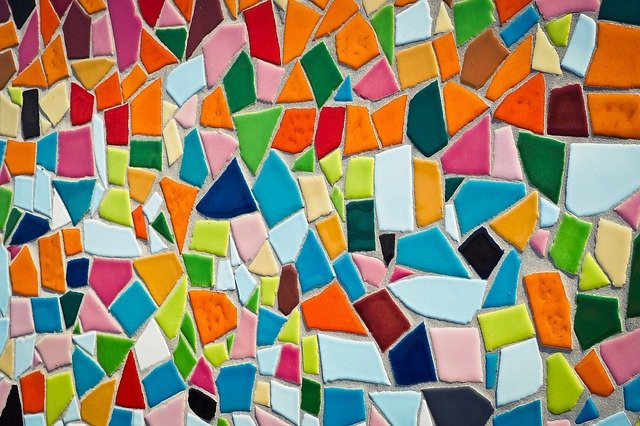
\includegraphics[scale=1.3]{pics/mosaic.jpg}}
		\caption{Mosaikbild (www.pixabay.com,\\ Fotograf: Michael Gaida)}
	\end{subfigure}\hfill
	\begin{subfigure}[t]{0.49\textwidth}
		\centering
		\boxed{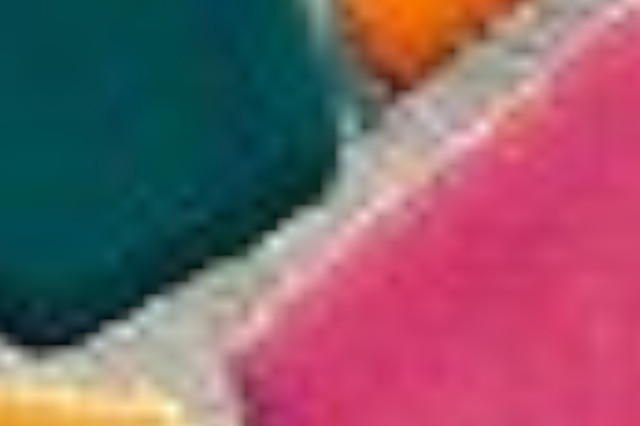
\includegraphics[scale=1.3]{pics/mosaic-zoom-20.jpg}}
		\caption{Mosaikbild bei 20-facher Vergrößerung}
	\end{subfigure}
	\caption{Bildskalierung unter Anwendung bilinearer Interpolation}
	\label{fig:MosaicBilinear}
\end{figure}
\noindent Wie im Ergebnisbild (b) zu erkennen, führt die lineare Interpolation dazu, das Kanten sehr unscharf und Strukturen verändert werden. Im Bereich der Materialstrukturanalyse, wie später in Kapitel \ref{sec:Problemstellung} auf Seite \pageref{sec:Problemstellung} noch gezeigt wird, kann das (auch bei wesentlich kleineren Skalierungsfaktoren) zu sehr unerwünschten Einflüssen führen und Messergebnisse verfälschen.
\\\\
\noindent\textbf{Nearest-Neighbor-Interpolation}
\\\\
Bei diesem Interpolationsverfahren wird ein etwas anderer Ansatz als der zuvor betrachtete verfolgt. Hierbei wird jedem Pixel im skalierten Ergebnisbild der Farbwert zugewiesen, der seinem nächsten Nachbarn im Originalbild entspricht. 
\\\\
Wie auch bei der linearen Interpolation, wird zunächst den Pixeln im Ergebnisbild, deren Position der um den Skalierungsfaktor $\lambda$ in X/Y-Richtung verschobenen 
Pixel im Originalbild entspricht, dessen Farbwert zugewiesen. In der nachstehenden Abbildung \ref{fig:NearestNeighborInterpolation} wurden diese entsprechend markiert. Das Originalbild ist identisch mit dem in Abbildung \ref{fig:BilinearInterpolation1} auf Seite \pageref{fig:BilinearInterpolation1} (links), wurde jedoch wegen der größeren Skalierung ($\lambda = 4$) aus Platzgründen hier nicht dargestellt.

\begin{figure}[H]
	\centering
	\begin{tikzpicture}[x=0.75pt,y=0.75pt,yscale=-1,xscale=1, scale=1.2, every node/.style={scale=1.2}]
		%uncomment if require: \path (0,374); %set diagram left start at 0, and has height of 374
		
		%Shape: Grid [id:dp7095227503573782] 
		\draw  [draw opacity=0][line width=1.5]  (184.38,71.85) -- (545.38,71.85) -- (545.38,432.85) -- (184.38,432.85) -- cycle ; \draw  [color={rgb, 255:red, 0; green, 0; blue, 0 }  ,draw opacity=1 ][line width=1.5]  (184.38,71.85) -- (184.38,432.85)(214.38,71.85) -- (214.38,432.85)(244.38,71.85) -- (244.38,432.85)(274.38,71.85) -- (274.38,432.85)(304.38,71.85) -- (304.38,432.85)(334.38,71.85) -- (334.38,432.85)(364.38,71.85) -- (364.38,432.85)(394.38,71.85) -- (394.38,432.85)(424.38,71.85) -- (424.38,432.85)(454.38,71.85) -- (454.38,432.85)(484.38,71.85) -- (484.38,432.85)(514.38,71.85) -- (514.38,432.85)(544.38,71.85) -- (544.38,432.85) ; \draw  [color={rgb, 255:red, 0; green, 0; blue, 0 }  ,draw opacity=1 ][line width=1.5]  (184.38,71.85) -- (545.38,71.85)(184.38,101.85) -- (545.38,101.85)(184.38,131.85) -- (545.38,131.85)(184.38,161.85) -- (545.38,161.85)(184.38,191.85) -- (545.38,191.85)(184.38,221.85) -- (545.38,221.85)(184.38,251.85) -- (545.38,251.85)(184.38,281.85) -- (545.38,281.85)(184.38,311.85) -- (545.38,311.85)(184.38,341.85) -- (545.38,341.85)(184.38,371.85) -- (545.38,371.85)(184.38,401.85) -- (545.38,401.85)(184.38,431.85) -- (545.38,431.85) ; \draw  [color={rgb, 255:red, 0; green, 0; blue, 0 }  ,draw opacity=1 ][line width=1.5]   ;
		%Shape: Axis 2D [id:dp8498955334043249] 
		\draw  (162.06,1.16) -- (162.06,462.85)(569.38,47.33) -- (116.81,47.33) (167.06,455.85) -- (162.06,462.85) -- (157.06,455.85) (562.38,42.33) -- (569.38,47.33) -- (562.38,52.33)  ;
		%Shape: Rectangle [id:dp03158858882810189] 
		\draw  [fill={rgb, 255:red, 245; green, 166; blue, 35 }  ,fill opacity=1 ][line width=1.5]  (304.38,71.85) -- (334.38,71.85) -- (334.38,101.85) -- (304.38,101.85) -- cycle ;
		%Shape: Rectangle [id:dp4293172616657537] 
		\draw  [fill={rgb, 255:red, 245; green, 166; blue, 35 }  ,fill opacity=1 ][line width=1.5]  (424.38,191.85) -- (454.38,191.85) -- (454.38,221.85) -- (424.38,221.85) -- cycle ;
		%Shape: Rectangle [id:dp7403667468656355] 
		\draw  [fill={rgb, 255:red, 126; green, 211; blue, 33 }  ,fill opacity=1 ][line width=1.5]  (424.38,71.85) -- (454.38,71.85) -- (454.38,101.85) -- (424.38,101.85) -- cycle ;
		%Shape: Rectangle [id:dp06224277384743582] 
		\draw  [fill={rgb, 255:red, 126; green, 211; blue, 33 }  ,fill opacity=1 ][line width=1.5]  (304.19,191.85) -- (334.19,191.85) -- (334.19,221.85) -- (304.19,221.85) -- cycle ;
		%Shape: Rectangle [id:dp7749039558596071] 
		\draw  [fill={rgb, 255:red, 126; green, 211; blue, 33 }  ,fill opacity=1 ][line width=1.5]  (184.38,71.85) -- (214.38,71.85) -- (214.38,101.85) -- (184.38,101.85) -- cycle ;
		%Shape: Rectangle [id:dp76695095788688] 
		\draw  [fill={rgb, 255:red, 126; green, 211; blue, 33 }  ,fill opacity=1 ][line width=1.5]  (184.38,221.85) -- (214.38,221.85) -- (214.38,251.85) -- (184.38,251.85) -- cycle ;
		%Shape: Rectangle [id:dp8501675458754504] 
		\draw  [fill={rgb, 255:red, 126; green, 211; blue, 33 }  ,fill opacity=1 ][line width=1.5]  (184.38,101.85) -- (214.38,101.85) -- (214.38,131.85) -- (184.38,131.85) -- cycle ;
		%Shape: Rectangle [id:dp3563846058181176] 
		\draw  [fill={rgb, 255:red, 126; green, 211; blue, 33 }  ,fill opacity=1 ][line width=1.5]  (184.38,191.85) -- (214.38,191.85) -- (214.38,221.85) -- (184.38,221.85) -- cycle ;
		%Shape: Rectangle [id:dp08038388586370382] 
		\draw  [fill={rgb, 255:red, 245; green, 166; blue, 35 }  ,fill opacity=1 ][line width=1.5]  (184.38,371.85) -- (214.38,371.85) -- (214.38,401.85) -- (184.38,401.85) -- cycle ;
		%Shape: Rectangle [id:dp17427156018316536] 
		\draw  [fill={rgb, 255:red, 245; green, 166; blue, 35 }  ,fill opacity=1 ][line width=1.5]  (184.38,401.85) -- (214.38,401.85) -- (214.38,431.85) -- (184.38,431.85) -- cycle ;
		%Shape: Rectangle [id:dp5230981929272401] 
		\draw  [fill={rgb, 255:red, 245; green, 166; blue, 35 }  ,fill opacity=1 ][line width=1.5]  (184.38,281.85) -- (214.38,281.85) -- (214.38,311.85) -- (184.38,311.85) -- cycle ;
		%Shape: Rectangle [id:dp8781386664034937] 
		\draw  [fill={rgb, 255:red, 245; green, 166; blue, 35 }  ,fill opacity=1 ][line width=1.5]  (184.38,311.85) -- (214.38,311.85) -- (214.38,341.85) -- (184.38,341.85) -- cycle ;
		%Shape: Rectangle [id:dp014315444147270817] 
		\draw  [fill={rgb, 255:red, 245; green, 166; blue, 35 }  ,fill opacity=1 ][line width=1.5]  (304.38,311.85) -- (334.38,311.85) -- (334.38,341.85) -- (304.38,341.85) -- cycle ;
		%Shape: Rectangle [id:dp4285755632512277] 
		\draw  [fill={rgb, 255:red, 245; green, 166; blue, 35 }  ,fill opacity=1 ][line width=1.5]  (304.38,281.85) -- (334.38,281.85) -- (334.38,311.85) -- (304.38,311.85) -- cycle ;
		%Shape: Rectangle [id:dp1815738184360829] 
		\draw  [fill={rgb, 255:red, 245; green, 166; blue, 35 }  ,fill opacity=1 ][line width=1.5]  (334.38,281.85) -- (364.38,281.85) -- (364.38,311.85) -- (334.38,311.85) -- cycle ;
		%Shape: Rectangle [id:dp9546918808720398] 
		\draw  [fill={rgb, 255:red, 245; green, 166; blue, 35 }  ,fill opacity=1 ][line width=1.5]  (394.38,281.85) -- (424.38,281.85) -- (424.38,311.85) -- (394.38,311.85) -- cycle ;
		%Shape: Rectangle [id:dp07796130206690832] 
		\draw  [fill={rgb, 255:red, 245; green, 166; blue, 35 }  ,fill opacity=1 ][line width=1.5]  (394.38,311.85) -- (424.38,311.85) -- (424.38,341.85) -- (394.38,341.85) -- cycle ;
		%Shape: Rectangle [id:dp18026278573351429] 
		\draw  [fill={rgb, 255:red, 245; green, 166; blue, 35 }  ,fill opacity=1 ][line width=1.5]  (424.38,281.85) -- (454.38,281.85) -- (454.38,311.85) -- (424.38,311.85) -- cycle ;
		%Shape: Rectangle [id:dp7464297643123727] 
		\draw  [fill={rgb, 255:red, 245; green, 166; blue, 35 }  ,fill opacity=1 ][line width=1.5]  (424.38,311.85) -- (454.38,311.85) -- (454.38,341.85) -- (424.38,341.85) -- cycle ;
		%Shape: Rectangle [id:dp8531876137714547] 
		\draw  [fill={rgb, 255:red, 185; green, 188; blue, 34 }  ,fill opacity=1 ][line width=1.5]  (244.38,71.85) -- (274.38,71.85) -- (274.38,101.85) -- (244.38,101.85) -- cycle ;
		%Shape: Rectangle [id:dp6306343414110546] 
		\draw  [fill={rgb, 255:red, 185; green, 188; blue, 34 }  ,fill opacity=1 ][line width=1.5]  (304.38,131.85) -- (334.38,131.85) -- (334.38,161.85) -- (304.38,161.85) -- cycle ;
		%Shape: Rectangle [id:dp259680405538511] 
		\draw  [fill={rgb, 255:red, 185; green, 188; blue, 34 }  ,fill opacity=1 ][line width=1.5]  (364.38,71.85) -- (394.38,71.85) -- (394.38,101.85) -- (364.38,101.85) -- cycle ;
		%Shape: Rectangle [id:dp2981542538583779] 
		\draw  [fill={rgb, 255:red, 185; green, 188; blue, 34 }  ,fill opacity=1 ][line width=1.5]  (424.38,131.85) -- (454.38,131.85) -- (454.38,161.85) -- (424.38,161.85) -- cycle ;
		%Shape: Rectangle [id:dp11287077393924216] 
		\draw  [fill={rgb, 255:red, 185; green, 188; blue, 34 }  ,fill opacity=1 ][line width=1.5]  (304.38,251.85) -- (334.38,251.85) -- (334.38,281.85) -- (304.38,281.85) -- cycle ;
		%Shape: Rectangle [id:dp34828348842093915] 
		\draw  [fill={rgb, 255:red, 185; green, 188; blue, 34 }  ,fill opacity=1 ][line width=1.5]  (184.38,251.85) -- (214.38,251.85) -- (214.38,281.85) -- (184.38,281.85) -- cycle ;
		%Shape: Rectangle [id:dp20967156569205625] 
		\draw  [fill={rgb, 255:red, 245; green, 166; blue, 35 }  ,fill opacity=1 ][line width=1.5]  (184.38,341.85) -- (214.38,341.85) -- (214.38,371.85) -- (184.38,371.85) -- cycle ;
		%Shape: Rectangle [id:dp8645622073796068] 
		\draw  [fill={rgb, 255:red, 245; green, 166; blue, 35 }  ,fill opacity=1 ][line width=1.5]  (214.38,371.85) -- (244.38,371.85) -- (244.38,401.85) -- (214.38,401.85) -- cycle ;
		%Shape: Rectangle [id:dp9231080124282475] 
		\draw  [fill={rgb, 255:red, 245; green, 166; blue, 35 }  ,fill opacity=1 ][line width=1.5]  (214.38,401.85) -- (244.38,401.85) -- (244.38,431.85) -- (214.38,431.85) -- cycle ;
		%Shape: Rectangle [id:dp6204877241605248] 
		\draw  [fill={rgb, 255:red, 245; green, 166; blue, 35 }  ,fill opacity=1 ][line width=1.5]  (214.38,341.85) -- (244.38,341.85) -- (244.38,371.85) -- (214.38,371.85) -- cycle ;
		%Shape: Rectangle [id:dp38032931107912693] 
		\draw  [fill={rgb, 255:red, 245; green, 166; blue, 35 }  ,fill opacity=1 ][line width=1.5]  (244.38,401.85) -- (274.38,401.85) -- (274.38,431.85) -- (244.38,431.85) -- cycle ;
		%Shape: Rectangle [id:dp8408404877468413] 
		\draw  [fill={rgb, 255:red, 245; green, 166; blue, 35 }  ,fill opacity=1 ][line width=1.5]  (274.38,401.85) -- (304.38,401.85) -- (304.38,431.85) -- (274.38,431.85) -- cycle ;
		%Shape: Rectangle [id:dp3790931654626404] 
		\draw  [fill={rgb, 255:red, 245; green, 166; blue, 35 }  ,fill opacity=1 ][line width=1.5]  (274.38,371.85) -- (304.38,371.85) -- (304.38,401.85) -- (274.38,401.85) -- cycle ;
		%Shape: Rectangle [id:dp8226385564330679] 
		\draw  [fill={rgb, 255:red, 245; green, 166; blue, 35 }  ,fill opacity=1 ][line width=1.5]  (274.38,341.85) -- (304.38,341.85) -- (304.38,371.85) -- (274.38,371.85) -- cycle ;
		%Shape: Rectangle [id:dp4824239487826214] 
		\draw  [fill={rgb, 255:red, 245; green, 166; blue, 35 }  ,fill opacity=1 ][line width=1.5]  (244.38,341.85) -- (274.38,341.85) -- (274.38,371.85) -- (244.38,371.85) -- cycle ;
		%Shape: Rectangle [id:dp8450066874115723] 
		\draw  [fill={rgb, 255:red, 245; green, 166; blue, 35 }  ,fill opacity=1 ][line width=1.5]  (244.38,371.85) -- (274.38,371.85) -- (274.38,401.85) -- (244.38,401.85) -- cycle ;
		%Shape: Rectangle [id:dp49854053727123826] 
		\draw  [fill={rgb, 255:red, 245; green, 166; blue, 35 }  ,fill opacity=1 ][line width=1.5]  (394.38,341.85) -- (424.38,341.85) -- (424.38,371.85) -- (394.38,371.85) -- cycle ;
		%Shape: Rectangle [id:dp2547398450949824] 
		\draw  [fill={rgb, 255:red, 245; green, 166; blue, 35 }  ,fill opacity=1 ][line width=1.5]  (364.38,401.85) -- (394.38,401.85) -- (394.38,431.85) -- (364.38,431.85) -- cycle ;
		%Shape: Rectangle [id:dp3397145262838692] 
		\draw  [fill={rgb, 255:red, 245; green, 166; blue, 35 }  ,fill opacity=1 ][line width=1.5]  (364.38,371.85) -- (394.38,371.85) -- (394.38,401.85) -- (364.38,401.85) -- cycle ;
		%Shape: Rectangle [id:dp4625714593708592] 
		\draw  [fill={rgb, 255:red, 245; green, 166; blue, 35 }  ,fill opacity=1 ][line width=1.5]  (364.38,341.85) -- (394.38,341.85) -- (394.38,371.85) -- (364.38,371.85) -- cycle ;
		%Shape: Rectangle [id:dp018560203340834858] 
		\draw  [fill={rgb, 255:red, 245; green, 166; blue, 35 }  ,fill opacity=1 ][line width=1.5]  (334.38,401.85) -- (364.38,401.85) -- (364.38,431.85) -- (334.38,431.85) -- cycle ;
		%Shape: Rectangle [id:dp8758131643785033] 
		\draw  [fill={rgb, 255:red, 245; green, 166; blue, 35 }  ,fill opacity=1 ][line width=1.5]  (334.38,371.85) -- (364.38,371.85) -- (364.38,401.85) -- (334.38,401.85) -- cycle ;
		%Shape: Rectangle [id:dp6045783736928364] 
		\draw  [fill={rgb, 255:red, 245; green, 166; blue, 35 }  ,fill opacity=1 ][line width=1.5]  (334.38,341.85) -- (364.38,341.85) -- (364.38,371.85) -- (334.38,371.85) -- cycle ;
		%Shape: Rectangle [id:dp8091061375318492] 
		\draw  [fill={rgb, 255:red, 245; green, 166; blue, 35 }  ,fill opacity=1 ][line width=1.5]  (304.38,401.85) -- (334.38,401.85) -- (334.38,431.85) -- (304.38,431.85) -- cycle ;
		%Shape: Rectangle [id:dp3619595141687527] 
		\draw  [fill={rgb, 255:red, 245; green, 166; blue, 35 }  ,fill opacity=1 ][line width=1.5]  (304.38,371.85) -- (334.38,371.85) -- (334.38,401.85) -- (304.38,401.85) -- cycle ;
		%Shape: Rectangle [id:dp3810282566587372] 
		\draw  [fill={rgb, 255:red, 245; green, 166; blue, 35 }  ,fill opacity=1 ][line width=1.5]  (304.38,341.85) -- (334.38,341.85) -- (334.38,371.85) -- (304.38,371.85) -- cycle ;
		%Shape: Rectangle [id:dp7070882796459546] 
		\draw  [fill={rgb, 255:red, 245; green, 166; blue, 35 }  ,fill opacity=1 ][line width=1.5]  (484.38,341.85) -- (514.38,341.85) -- (514.38,371.85) -- (484.38,371.85) -- cycle ;
		%Shape: Rectangle [id:dp09438757715247048] 
		\draw  [fill={rgb, 255:red, 245; green, 166; blue, 35 }  ,fill opacity=1 ][line width=1.5]  (454.38,341.85) -- (484.38,341.85) -- (484.38,371.85) -- (454.38,371.85) -- cycle ;
		%Shape: Rectangle [id:dp8797072531264896] 
		\draw  [fill={rgb, 255:red, 245; green, 166; blue, 35 }  ,fill opacity=1 ][line width=1.5]  (454.38,371.85) -- (484.38,371.85) -- (484.38,401.85) -- (454.38,401.85) -- cycle ;
		%Shape: Rectangle [id:dp5564013956674208] 
		\draw  [fill={rgb, 255:red, 245; green, 166; blue, 35 }  ,fill opacity=1 ][line width=1.5]  (454.38,401.85) -- (484.38,401.85) -- (484.38,431.85) -- (454.38,431.85) -- cycle ;
		%Shape: Rectangle [id:dp966247624331478] 
		\draw  [fill={rgb, 255:red, 245; green, 166; blue, 35 }  ,fill opacity=1 ][line width=1.5]  (424.38,401.85) -- (454.38,401.85) -- (454.38,431.85) -- (424.38,431.85) -- cycle ;
		%Shape: Rectangle [id:dp29279739542535255] 
		\draw  [fill={rgb, 255:red, 245; green, 166; blue, 35 }  ,fill opacity=1 ][line width=1.5]  (424.38,371.85) -- (454.38,371.85) -- (454.38,401.85) -- (424.38,401.85) -- cycle ;
		%Shape: Rectangle [id:dp09431481081749615] 
		\draw  [fill={rgb, 255:red, 245; green, 166; blue, 35 }  ,fill opacity=1 ][line width=1.5]  (424.38,341.85) -- (454.38,341.85) -- (454.38,371.85) -- (424.38,371.85) -- cycle ;
		%Shape: Rectangle [id:dp37445774068642135] 
		\draw  [fill={rgb, 255:red, 245; green, 166; blue, 35 }  ,fill opacity=1 ][line width=1.5]  (394.38,401.85) -- (424.38,401.85) -- (424.38,431.85) -- (394.38,431.85) -- cycle ;
		%Shape: Rectangle [id:dp6941244471773985] 
		\draw  [fill={rgb, 255:red, 245; green, 166; blue, 35 }  ,fill opacity=1 ][line width=1.5]  (394.38,371.85) -- (424.38,371.85) -- (424.38,401.85) -- (394.38,401.85) -- cycle ;
		%Shape: Rectangle [id:dp31276694034774954] 
		\draw  [fill={rgb, 255:red, 245; green, 166; blue, 35 }  ,fill opacity=1 ][line width=1.5]  (514.38,401.85) -- (544.38,401.85) -- (544.38,431.85) -- (514.38,431.85) -- cycle ;
		%Shape: Rectangle [id:dp9772583055839423] 
		\draw  [fill={rgb, 255:red, 245; green, 166; blue, 35 }  ,fill opacity=1 ][line width=1.5]  (514.38,371.85) -- (544.38,371.85) -- (544.38,401.85) -- (514.38,401.85) -- cycle ;
		%Shape: Rectangle [id:dp6064399230528661] 
		\draw  [fill={rgb, 255:red, 245; green, 166; blue, 35 }  ,fill opacity=1 ][line width=1.5]  (514.38,341.85) -- (544.38,341.85) -- (544.38,371.85) -- (514.38,371.85) -- cycle ;
		%Shape: Rectangle [id:dp5886691875587856] 
		\draw  [fill={rgb, 255:red, 245; green, 166; blue, 35 }  ,fill opacity=1 ][line width=1.5]  (484.38,401.85) -- (514.38,401.85) -- (514.38,431.85) -- (484.38,431.85) -- cycle ;
		%Shape: Rectangle [id:dp8046657763586618] 
		\draw  [fill={rgb, 255:red, 245; green, 166; blue, 35 }  ,fill opacity=1 ][line width=1.5]  (484.38,371.85) -- (514.38,371.85) -- (514.38,401.85) -- (484.38,401.85) -- cycle ;
		%Shape: Rectangle [id:dp15837309002405686] 
		\draw  [fill={rgb, 255:red, 126; green, 211; blue, 33 }  ,fill opacity=1 ][line width=1.5]  (214.19,191.85) -- (244.19,191.85) -- (244.19,221.85) -- (214.19,221.85) -- cycle ;
		%Shape: Rectangle [id:dp7661776980019065] 
		\draw  [fill={rgb, 255:red, 126; green, 211; blue, 33 }  ,fill opacity=1 ][line width=1.5]  (244.19,191.85) -- (274.19,191.85) -- (274.19,221.85) -- (244.19,221.85) -- cycle ;
		%Shape: Rectangle [id:dp4715704882749524] 
		\draw  [fill={rgb, 255:red, 126; green, 211; blue, 33 }  ,fill opacity=1 ][line width=1.5]  (274.19,191.85) -- (304.19,191.85) -- (304.19,221.85) -- (274.19,221.85) -- cycle ;
		%Shape: Rectangle [id:dp19487499668887354] 
		\draw  [fill={rgb, 255:red, 126; green, 211; blue, 33 }  ,fill opacity=1 ][line width=1.5]  (334.19,191.85) -- (364.19,191.85) -- (364.19,221.85) -- (334.19,221.85) -- cycle ;
		%Shape: Rectangle [id:dp8242877674588471] 
		\draw  [fill={rgb, 255:red, 245; green, 166; blue, 35 }  ,fill opacity=1 ][line width=1.5]  (394.38,191.85) -- (424.38,191.85) -- (424.38,221.85) -- (394.38,221.85) -- cycle ;
		%Shape: Rectangle [id:dp9239067903223326] 
		\draw  [fill={rgb, 255:red, 245; green, 166; blue, 35 }  ,fill opacity=1 ][line width=1.5]  (424.38,251.85) -- (454.38,251.85) -- (454.38,281.85) -- (424.38,281.85) -- cycle ;
		%Shape: Rectangle [id:dp019140055117673582] 
		\draw  [fill={rgb, 255:red, 245; green, 166; blue, 35 }  ,fill opacity=1 ][line width=1.5]  (514.38,251.85) -- (544.38,251.85) -- (544.38,281.85) -- (514.38,281.85) -- cycle ;
		%Shape: Rectangle [id:dp24400311996228086] 
		\draw  [fill={rgb, 255:red, 245; green, 166; blue, 35 }  ,fill opacity=1 ][line width=1.5]  (484.38,251.85) -- (514.38,251.85) -- (514.38,281.85) -- (484.38,281.85) -- cycle ;
		%Shape: Rectangle [id:dp6537695625446079] 
		\draw  [fill={rgb, 255:red, 245; green, 166; blue, 35 }  ,fill opacity=1 ][line width=1.5]  (454.38,251.85) -- (484.38,251.85) -- (484.38,281.85) -- (454.38,281.85) -- cycle ;
		%Shape: Rectangle [id:dp347234781940998] 
		\draw  [fill={rgb, 255:red, 245; green, 166; blue, 35 }  ,fill opacity=1 ][line width=1.5]  (424.38,221.85) -- (454.38,221.85) -- (454.38,251.85) -- (424.38,251.85) -- cycle ;
		%Shape: Rectangle [id:dp8436434674198796] 
		\draw  [fill={rgb, 255:red, 245; green, 166; blue, 35 }  ,fill opacity=1 ][line width=1.5]  (514.38,221.85) -- (544.38,221.85) -- (544.38,251.85) -- (514.38,251.85) -- cycle ;
		%Shape: Rectangle [id:dp20066804981766095] 
		\draw  [fill={rgb, 255:red, 245; green, 166; blue, 35 }  ,fill opacity=1 ][line width=1.5]  (484.38,221.85) -- (514.38,221.85) -- (514.38,251.85) -- (484.38,251.85) -- cycle ;
		%Shape: Rectangle [id:dp19586197595653332] 
		\draw  [fill={rgb, 255:red, 245; green, 166; blue, 35 }  ,fill opacity=1 ][line width=1.5]  (454.38,221.85) -- (484.38,221.85) -- (484.38,251.85) -- (454.38,251.85) -- cycle ;
		%Shape: Rectangle [id:dp15661261486124634] 
		\draw  [fill={rgb, 255:red, 245; green, 166; blue, 35 }  ,fill opacity=1 ][line width=1.5]  (484.38,281.85) -- (514.38,281.85) -- (514.38,311.85) -- (484.38,311.85) -- cycle ;
		%Shape: Rectangle [id:dp8422930977209842] 
		\draw  [fill={rgb, 255:red, 245; green, 166; blue, 35 }  ,fill opacity=1 ][line width=1.5]  (454.38,281.85) -- (484.38,281.85) -- (484.38,311.85) -- (454.38,311.85) -- cycle ;
		%Shape: Rectangle [id:dp533726390813522] 
		\draw  [fill={rgb, 255:red, 245; green, 166; blue, 35 }  ,fill opacity=1 ][line width=1.5]  (514.38,281.85) -- (544.38,281.85) -- (544.38,311.85) -- (514.38,311.85) -- cycle ;
		%Shape: Rectangle [id:dp7594285250318692] 
		\draw  [fill={rgb, 255:red, 245; green, 166; blue, 35 }  ,fill opacity=1 ][line width=1.5]  (484.38,311.85) -- (514.38,311.85) -- (514.38,341.85) -- (484.38,341.85) -- cycle ;
		%Shape: Rectangle [id:dp6017798318891361] 
		\draw  [fill={rgb, 255:red, 245; green, 166; blue, 35 }  ,fill opacity=1 ][line width=1.5]  (454.38,311.85) -- (484.38,311.85) -- (484.38,341.85) -- (454.38,341.85) -- cycle ;
		%Shape: Rectangle [id:dp6032372566019569] 
		\draw  [fill={rgb, 255:red, 245; green, 166; blue, 35 }  ,fill opacity=1 ][line width=1.5]  (514.38,311.85) -- (544.38,311.85) -- (544.38,341.85) -- (514.38,341.85) -- cycle ;
		%Shape: Rectangle [id:dp7556768506148435] 
		\draw  [fill={rgb, 255:red, 245; green, 166; blue, 35 }  ,fill opacity=1 ][line width=1.5]  (484.38,191.85) -- (514.38,191.85) -- (514.38,221.85) -- (484.38,221.85) -- cycle ;
		%Shape: Rectangle [id:dp5763577241712744] 
		\draw  [fill={rgb, 255:red, 245; green, 166; blue, 35 }  ,fill opacity=1 ][line width=1.5]  (454.38,191.85) -- (484.38,191.85) -- (484.38,221.85) -- (454.38,221.85) -- cycle ;
		%Shape: Rectangle [id:dp9410445845457768] 
		\draw  [fill={rgb, 255:red, 245; green, 166; blue, 35 }  ,fill opacity=1 ][line width=1.5]  (514.38,191.85) -- (544.38,191.85) -- (544.38,221.85) -- (514.38,221.85) -- cycle ;
		%Shape: Rectangle [id:dp40670546903890026] 
		\draw  [fill={rgb, 255:red, 185; green, 188; blue, 34 }  ,fill opacity=1 ][line width=1.5]  (244.38,251.85) -- (274.38,251.85) -- (274.38,281.85) -- (244.38,281.85) -- cycle ;
		%Shape: Rectangle [id:dp8977108078911407] 
		\draw  [fill={rgb, 255:red, 245; green, 166; blue, 35 }  ,fill opacity=1 ][line width=1.5]  (334.38,311.85) -- (364.38,311.85) -- (364.38,341.85) -- (334.38,341.85) -- cycle ;
		%Shape: Rectangle [id:dp7074431973385585] 
		\draw  [fill={rgb, 255:red, 245; green, 166; blue, 35 }  ,fill opacity=1 ][line width=1.5]  (364.38,311.85) -- (394.38,311.85) -- (394.38,341.85) -- (364.38,341.85) -- cycle ;
		%Shape: Rectangle [id:dp02442010256765048] 
		\draw  [fill={rgb, 255:red, 245; green, 166; blue, 35 }  ,fill opacity=1 ][line width=1.5]  (244.38,311.85) -- (274.38,311.85) -- (274.38,341.85) -- (244.38,341.85) -- cycle ;
		%Shape: Rectangle [id:dp7698025639540884] 
		\draw  [fill={rgb, 255:red, 245; green, 166; blue, 35 }  ,fill opacity=1 ][line width=1.5]  (214.38,311.85) -- (244.38,311.85) -- (244.38,341.85) -- (214.38,341.85) -- cycle ;
		%Shape: Rectangle [id:dp05928417793438712] 
		\draw  [fill={rgb, 255:red, 245; green, 166; blue, 35 }  ,fill opacity=1 ][line width=1.5]  (274.38,311.85) -- (304.38,311.85) -- (304.38,341.85) -- (274.38,341.85) -- cycle ;
		%Shape: Rectangle [id:dp17903596454579307] 
		\draw  [fill={rgb, 255:red, 245; green, 166; blue, 35 }  ,fill opacity=1 ][line width=1.5]  (394.38,161.85) -- (424.38,161.85) -- (424.38,191.85) -- (394.38,191.85) -- cycle ;
		%Shape: Rectangle [id:dp6818574603589049] 
		\draw  [fill={rgb, 255:red, 245; green, 166; blue, 35 }  ,fill opacity=1 ][line width=1.5]  (214.38,281.85) -- (244.38,281.85) -- (244.38,311.85) -- (214.38,311.85) -- cycle ;
		%Shape: Rectangle [id:dp06291493751997224] 
		\draw  [fill={rgb, 255:red, 245; green, 166; blue, 35 }  ,fill opacity=1 ][line width=1.5]  (244.38,281.85) -- (274.38,281.85) -- (274.38,311.85) -- (244.38,311.85) -- cycle ;
		%Shape: Rectangle [id:dp7550031462325714] 
		\draw  [fill={rgb, 255:red, 245; green, 166; blue, 35 }  ,fill opacity=1 ][line width=1.5]  (274.38,281.85) -- (304.38,281.85) -- (304.38,311.85) -- (274.38,311.85) -- cycle ;
		%Shape: Rectangle [id:dp6238172864997027] 
		\draw  [fill={rgb, 255:red, 245; green, 166; blue, 35 }  ,fill opacity=1 ][line width=1.5]  (364.38,281.85) -- (394.38,281.85) -- (394.38,311.85) -- (364.38,311.85) -- cycle ;
		%Shape: Rectangle [id:dp07628594409081513] 
		\draw  [fill={rgb, 255:red, 185; green, 188; blue, 34 }  ,fill opacity=1 ][line width=1.5]  (334.38,251.85) -- (364.38,251.85) -- (364.38,281.85) -- (334.38,281.85) -- cycle ;
		%Shape: Rectangle [id:dp9563558866695636] 
		\draw  [fill={rgb, 255:red, 185; green, 188; blue, 34 }  ,fill opacity=1 ][line width=1.5]  (274.38,251.85) -- (304.38,251.85) -- (304.38,281.85) -- (274.38,281.85) -- cycle ;
		%Shape: Rectangle [id:dp34871218697661277] 
		\draw  [fill={rgb, 255:red, 185; green, 188; blue, 34 }  ,fill opacity=1 ][line width=1.5]  (214.38,251.85) -- (244.38,251.85) -- (244.38,281.85) -- (214.38,281.85) -- cycle ;
		%Shape: Rectangle [id:dp5361925931463092] 
		\draw  [fill={rgb, 255:red, 245; green, 166; blue, 35 }  ,fill opacity=1 ][line width=1.5]  (394.38,251.85) -- (424.38,251.85) -- (424.38,281.85) -- (394.38,281.85) -- cycle ;
		%Shape: Rectangle [id:dp5518929265219127] 
		\draw  [fill={rgb, 255:red, 245; green, 166; blue, 35 }  ,fill opacity=1 ][line width=1.5]  (394.38,221.85) -- (424.38,221.85) -- (424.38,251.85) -- (394.38,251.85) -- cycle ;
		%Shape: Rectangle [id:dp7537098161537151] 
		\draw  [fill={rgb, 255:red, 185; green, 188; blue, 34 }  ,fill opacity=1 ][line width=1.5]  (364.19,221.85) -- (394.19,221.85) -- (394.19,251.85) -- (364.19,251.85) -- cycle ;
		%Shape: Rectangle [id:dp502161029745532] 
		\draw  [fill={rgb, 255:red, 126; green, 211; blue, 33 }  ,fill opacity=1 ][line width=1.5]  (214.19,221.85) -- (244.19,221.85) -- (244.19,251.85) -- (214.19,251.85) -- cycle ;
		%Shape: Rectangle [id:dp4067843103060319] 
		\draw  [fill={rgb, 255:red, 126; green, 211; blue, 33 }  ,fill opacity=1 ][line width=1.5]  (244.19,221.85) -- (274.19,221.85) -- (274.19,251.85) -- (244.19,251.85) -- cycle ;
		%Shape: Rectangle [id:dp9407025523047791] 
		\draw  [fill={rgb, 255:red, 126; green, 211; blue, 33 }  ,fill opacity=1 ][line width=1.5]  (274.19,221.85) -- (304.19,221.85) -- (304.19,251.85) -- (274.19,251.85) -- cycle ;
		%Shape: Rectangle [id:dp8373771611597205] 
		\draw  [fill={rgb, 255:red, 126; green, 211; blue, 33 }  ,fill opacity=1 ][line width=1.5]  (304.19,221.85) -- (334.19,221.85) -- (334.19,251.85) -- (304.19,251.85) -- cycle ;
		%Shape: Rectangle [id:dp1909517118919084] 
		\draw  [fill={rgb, 255:red, 126; green, 211; blue, 33 }  ,fill opacity=1 ][line width=1.5]  (304.19,161.85) -- (334.19,161.85) -- (334.19,191.85) -- (304.19,191.85) -- cycle ;
		%Shape: Rectangle [id:dp24721105642959074] 
		\draw  [fill={rgb, 255:red, 126; green, 211; blue, 33 }  ,fill opacity=1 ][line width=1.5]  (214.19,161.85) -- (244.19,161.85) -- (244.19,191.85) -- (214.19,191.85) -- cycle ;
		%Shape: Rectangle [id:dp4818010949588952] 
		\draw  [fill={rgb, 255:red, 126; green, 211; blue, 33 }  ,fill opacity=1 ][line width=1.5]  (244.19,161.85) -- (274.19,161.85) -- (274.19,191.85) -- (244.19,191.85) -- cycle ;
		%Shape: Rectangle [id:dp8913295885308947] 
		\draw  [fill={rgb, 255:red, 126; green, 211; blue, 33 }  ,fill opacity=1 ][line width=1.5]  (274.19,161.85) -- (304.19,161.85) -- (304.19,191.85) -- (274.19,191.85) -- cycle ;
		%Shape: Rectangle [id:dp12699381078898309] 
		\draw  [fill={rgb, 255:red, 126; green, 211; blue, 33 }  ,fill opacity=1 ][line width=1.5]  (334.19,161.85) -- (364.19,161.85) -- (364.19,191.85) -- (334.19,191.85) -- cycle ;
		%Shape: Rectangle [id:dp48588782329332236] 
		\draw  [fill={rgb, 255:red, 185; green, 188; blue, 34 }  ,fill opacity=1 ][line width=1.5]  (364.38,161.85) -- (394.38,161.85) -- (394.38,191.85) -- (364.38,191.85) -- cycle ;
		%Shape: Rectangle [id:dp19503814460397373] 
		\draw  [fill={rgb, 255:red, 185; green, 188; blue, 34 }  ,fill opacity=1 ][line width=1.5]  (334.38,131.85) -- (364.38,131.85) -- (364.38,161.85) -- (334.38,161.85) -- cycle ;
		%Shape: Rectangle [id:dp023576258240981085] 
		\draw  [fill={rgb, 255:red, 185; green, 188; blue, 34 }  ,fill opacity=1 ][line width=1.5]  (364.38,131.85) -- (394.38,131.85) -- (394.38,161.85) -- (364.38,161.85) -- cycle ;
		%Shape: Rectangle [id:dp0271391855966836] 
		\draw  [fill={rgb, 255:red, 185; green, 188; blue, 34 }  ,fill opacity=1 ][line width=1.5]  (274.38,131.85) -- (304.38,131.85) -- (304.38,161.85) -- (274.38,161.85) -- cycle ;
		%Shape: Rectangle [id:dp35781442980599276] 
		\draw  [fill={rgb, 255:red, 126; green, 211; blue, 33 }  ,fill opacity=1 ][line width=1.5]  (184.38,131.85) -- (214.38,131.85) -- (214.38,161.85) -- (184.38,161.85) -- cycle ;
		%Shape: Rectangle [id:dp9077885895218637] 
		\draw  [fill={rgb, 255:red, 126; green, 211; blue, 33 }  ,fill opacity=1 ][line width=1.5]  (214.19,101.85) -- (244.19,101.85) -- (244.19,131.85) -- (214.19,131.85) -- cycle ;
		%Shape: Rectangle [id:dp11750094713798942] 
		\draw  [fill={rgb, 255:red, 126; green, 211; blue, 33 }  ,fill opacity=1 ][line width=1.5]  (214.19,131.85) -- (244.19,131.85) -- (244.19,161.85) -- (214.19,161.85) -- cycle ;
		%Shape: Rectangle [id:dp8220631433654678] 
		\draw  [fill={rgb, 255:red, 126; green, 211; blue, 33 }  ,fill opacity=1 ][line width=1.5]  (214.19,71.85) -- (244.19,71.85) -- (244.19,101.85) -- (214.19,101.85) -- cycle ;
		%Shape: Rectangle [id:dp2675805273049193] 
		\draw  [fill={rgb, 255:red, 185; green, 188; blue, 34 }  ,fill opacity=1 ][line width=1.5]  (394.38,131.85) -- (424.38,131.85) -- (424.38,161.85) -- (394.38,161.85) -- cycle ;
		%Shape: Rectangle [id:dp08022989531540003] 
		\draw  [fill={rgb, 255:red, 126; green, 211; blue, 33 }  ,fill opacity=1 ][line width=1.5]  (424.38,101.85) -- (454.38,101.85) -- (454.38,131.85) -- (424.38,131.85) -- cycle ;
		%Shape: Rectangle [id:dp10810860175748516] 
		\draw  [fill={rgb, 255:red, 126; green, 211; blue, 33 }  ,fill opacity=1 ][line width=1.5]  (394.38,71.85) -- (424.38,71.85) -- (424.38,101.85) -- (394.38,101.85) -- cycle ;
		%Shape: Rectangle [id:dp5443529585116083] 
		\draw  [fill={rgb, 255:red, 126; green, 211; blue, 33 }  ,fill opacity=1 ][line width=1.5]  (394.38,101.85) -- (424.38,101.85) -- (424.38,131.85) -- (394.38,131.85) -- cycle ;
		%Shape: Rectangle [id:dp6599464049478758] 
		\draw  [fill={rgb, 255:red, 126; green, 211; blue, 33 }  ,fill opacity=1 ][line width=1.5]  (514.38,101.85) -- (544.38,101.85) -- (544.38,131.85) -- (514.38,131.85) -- cycle ;
		%Shape: Rectangle [id:dp8869823220630783] 
		\draw  [fill={rgb, 255:red, 126; green, 211; blue, 33 }  ,fill opacity=1 ][line width=1.5]  (484.38,101.85) -- (514.38,101.85) -- (514.38,131.85) -- (484.38,131.85) -- cycle ;
		%Shape: Rectangle [id:dp9204136129951822] 
		\draw  [fill={rgb, 255:red, 126; green, 211; blue, 33 }  ,fill opacity=1 ][line width=1.5]  (454.38,101.85) -- (484.38,101.85) -- (484.38,131.85) -- (454.38,131.85) -- cycle ;
		%Shape: Rectangle [id:dp5658525510990897] 
		\draw  [fill={rgb, 255:red, 126; green, 211; blue, 33 }  ,fill opacity=1 ][line width=1.5]  (514.38,71.85) -- (544.38,71.85) -- (544.38,101.85) -- (514.38,101.85) -- cycle ;
		%Shape: Rectangle [id:dp3657036504107076] 
		\draw  [fill={rgb, 255:red, 126; green, 211; blue, 33 }  ,fill opacity=1 ][line width=1.5]  (484.38,71.85) -- (514.38,71.85) -- (514.38,101.85) -- (484.38,101.85) -- cycle ;
		%Shape: Rectangle [id:dp6087607261872113] 
		\draw  [fill={rgb, 255:red, 126; green, 211; blue, 33 }  ,fill opacity=1 ][line width=1.5]  (454.38,71.85) -- (484.38,71.85) -- (484.38,101.85) -- (454.38,101.85) -- cycle ;
		%Shape: Rectangle [id:dp5734954377108985] 
		\draw  [fill={rgb, 255:red, 185; green, 188; blue, 34 }  ,fill opacity=1 ][line width=1.5]  (514.38,131.85) -- (544.38,131.85) -- (544.38,161.85) -- (514.38,161.85) -- cycle ;
		%Shape: Rectangle [id:dp5218668783318545] 
		\draw  [fill={rgb, 255:red, 185; green, 188; blue, 34 }  ,fill opacity=1 ][line width=1.5]  (484.38,131.85) -- (514.38,131.85) -- (514.38,161.85) -- (484.38,161.85) -- cycle ;
		%Shape: Rectangle [id:dp9610987839197175] 
		\draw  [fill={rgb, 255:red, 185; green, 188; blue, 34 }  ,fill opacity=1 ][line width=1.5]  (454.38,131.85) -- (484.38,131.85) -- (484.38,161.85) -- (454.38,161.85) -- cycle ;
		%Shape: Rectangle [id:dp8010612057630523] 
		\draw  [fill={rgb, 255:red, 245; green, 166; blue, 35 }  ,fill opacity=1 ][line width=1.5]  (514.38,161.85) -- (544.38,161.85) -- (544.38,191.85) -- (514.38,191.85) -- cycle ;
		%Shape: Rectangle [id:dp09604187704189282] 
		\draw  [fill={rgb, 255:red, 245; green, 166; blue, 35 }  ,fill opacity=1 ][line width=1.5]  (484.38,161.85) -- (514.38,161.85) -- (514.38,191.85) -- (484.38,191.85) -- cycle ;
		%Shape: Rectangle [id:dp3043186676901124] 
		\draw  [fill={rgb, 255:red, 245; green, 166; blue, 35 }  ,fill opacity=1 ][line width=1.5]  (454.38,161.85) -- (484.38,161.85) -- (484.38,191.85) -- (454.38,191.85) -- cycle ;
		%Shape: Rectangle [id:dp9602638367166756] 
		\draw  [fill={rgb, 255:red, 245; green, 166; blue, 35 }  ,fill opacity=1 ][line width=1.5]  (424.38,161.85) -- (454.38,161.85) -- (454.38,191.85) -- (424.38,191.85) -- cycle ;
		%Shape: Rectangle [id:dp28533019470341425] 
		\draw  [fill={rgb, 255:red, 245; green, 166; blue, 35 }  ,fill opacity=1 ][line width=1.5]  (304.38,101.85) -- (334.38,101.85) -- (334.38,131.85) -- (304.38,131.85) -- cycle ;
		%Shape: Rectangle [id:dp951668993225821] 
		\draw  [fill={rgb, 255:red, 245; green, 166; blue, 35 }  ,fill opacity=1 ][line width=1.5]  (274.38,71.85) -- (304.38,71.85) -- (304.38,101.85) -- (274.38,101.85) -- cycle ;
		%Shape: Rectangle [id:dp7574624719567788] 
		\draw  [fill={rgb, 255:red, 245; green, 166; blue, 35 }  ,fill opacity=1 ][line width=1.5]  (334.38,71.85) -- (364.38,71.85) -- (364.38,101.85) -- (334.38,101.85) -- cycle ;
		%Shape: Rectangle [id:dp035531849024908246] 
		\draw  [fill={rgb, 255:red, 245; green, 166; blue, 35 }  ,fill opacity=1 ][line width=1.5]  (274.38,101.85) -- (304.38,101.85) -- (304.38,131.85) -- (274.38,131.85) -- cycle ;
		%Shape: Rectangle [id:dp17671235765503068] 
		\draw  [fill={rgb, 255:red, 245; green, 166; blue, 35 }  ,fill opacity=1 ][line width=1.5]  (334.38,101.85) -- (364.38,101.85) -- (364.38,131.85) -- (334.38,131.85) -- cycle ;
		%Shape: Rectangle [id:dp4451383323311112] 
		\draw  [fill={rgb, 255:red, 185; green, 188; blue, 34 }  ,fill opacity=1 ][line width=1.5]  (364.38,101.85) -- (394.38,101.85) -- (394.38,131.85) -- (364.38,131.85) -- cycle ;
		%Shape: Rectangle [id:dp4967793824170166] 
		\draw  [fill={rgb, 255:red, 185; green, 188; blue, 34 }  ,fill opacity=1 ][line width=1.5]  (244.38,101.85) -- (274.38,101.85) -- (274.38,131.85) -- (244.38,131.85) -- cycle ;
		%Shape: Rectangle [id:dp5039047829251926] 
		\draw  [fill={rgb, 255:red, 126; green, 211; blue, 33 }  ,fill opacity=1 ][line width=1.5]  (184.38,161.85) -- (214.38,161.85) -- (214.38,191.85) -- (184.38,191.85) -- cycle ;
		%Shape: Rectangle [id:dp33060559451821936] 
		\draw  [fill={rgb, 255:red, 155; green, 199; blue, 33 }  ,fill opacity=1 ][line width=1.5]  (244.38,131.85) -- (274.38,131.85) -- (274.38,161.85) -- (244.38,161.85) -- cycle ;
		%Shape: Rectangle [id:dp5766273074112415] 
		\draw  [fill={rgb, 255:red, 126; green, 211; blue, 33 }  ,fill opacity=1 ][line width=1.5]  (334.38,221.85) -- (364.38,221.85) -- (364.38,251.85) -- (334.38,251.85) -- cycle ;
		%Shape: Rectangle [id:dp7540542834520386] 
		\draw  [fill={rgb, 255:red, 185; green, 188; blue, 34 }  ,fill opacity=1 ][line width=1.5]  (364.38,191.85) -- (394.38,191.85) -- (394.38,221.85) -- (364.38,221.85) -- cycle ;
		%Shape: Rectangle [id:dp15234189410875232] 
		\draw  [fill={rgb, 255:red, 185; green, 188; blue, 34 }  ,fill opacity=1 ][line width=1.5]  (364.38,251.85) -- (394.38,251.85) -- (394.38,281.85) -- (364.38,281.85) -- cycle ;
		
		% Text Node
		\draw (134.98,271.99) node [anchor=north west][inner sep=0.75pt]  [font=\normalsize,rotate=-270.08] [align=left] {$\displaystyle \lambda \cdot \ y$};
		% Text Node
		\draw (347.56,26.98) node [anchor=north west][inner sep=0.75pt]  [font=\normalsize,rotate=-359.4] [align=left] {\textcolor[rgb]{0,0,0}{$\displaystyle \lambda \cdot \ x$}};
		% Text Node
		\draw (193,54) node [anchor=north west][inner sep=0.75pt]   [align=left] {0};
		% Text Node
		\draw (224,54) node [anchor=north west][inner sep=0.75pt]   [align=left] {1};
		% Text Node
		\draw (255,54) node [anchor=north west][inner sep=0.75pt]   [align=left] {2};
		% Text Node
		\draw (282,54) node [anchor=north west][inner sep=0.75pt]   [align=left] {3};
		% Text Node
		\draw (315,54) node [anchor=north west][inner sep=0.75pt]   [align=left] {4};
		% Text Node
		\draw (172,79) node [anchor=north west][inner sep=0.75pt]   [align=left] {0};
		% Text Node
		\draw (172,110) node [anchor=north west][inner sep=0.75pt]   [align=left] {1};
		% Text Node
		\draw (172,140) node [anchor=north west][inner sep=0.75pt]   [align=left] {2};
		% Text Node
		\draw (172,169) node [anchor=north west][inner sep=0.75pt]   [align=left] {3};
		% Text Node
		\draw (172,200) node [anchor=north west][inner sep=0.75pt]   [align=left] {4};
		% Text Node
		\draw (574,43) node [anchor=north west][inner sep=0.75pt]   [align=left] {x};
		% Text Node
		\draw (157,467) node [anchor=north west][inner sep=0.75pt]   [align=left] {y};
		% Text Node
		\draw (342,54) node [anchor=north west][inner sep=0.75pt]   [align=left] {5};
		% Text Node
		\draw (172,230) node [anchor=north west][inner sep=0.75pt]   [align=left] {5};
		% Text Node
		\draw (185,81) node [anchor=north west][inner sep=0.75pt]  [font=\scriptsize] [align=left] {$\displaystyle P_{( 0,0)}$};
		% Text Node
		\draw (305,81) node [anchor=north west][inner sep=0.75pt]  [font=\scriptsize] [align=left] {$\displaystyle P_{( 0,2)}$};
		% Text Node
		\draw (425,81) node [anchor=north west][inner sep=0.75pt]  [font=\scriptsize] [align=left] {$\displaystyle P_{( 0,4)}$};
		% Text Node
		\draw (185,201) node [anchor=north west][inner sep=0.75pt]  [font=\scriptsize] [align=left] {$\displaystyle P_{( 2,0)}$};
		% Text Node
		\draw (305,201) node [anchor=north west][inner sep=0.75pt]  [font=\scriptsize] [align=left] {$\displaystyle P_{( 2,2)}$};
		% Text Node
		\draw (425,201) node [anchor=north west][inner sep=0.75pt]  [font=\scriptsize] [align=left] {$\displaystyle P_{( 2,4)}$};
		% Text Node
		\draw (185,320) node [anchor=north west][inner sep=0.75pt]  [font=\scriptsize] [align=left] {$\displaystyle P_{( 4,0)}$};
		% Text Node
		\draw (305,320) node [anchor=north west][inner sep=0.75pt]  [font=\scriptsize] [align=left] {$\displaystyle P_{( 4,2)}$};
		% Text Node
		\draw (425,320) node [anchor=north west][inner sep=0.75pt]  [font=\scriptsize] [align=left] {$\displaystyle P_{( 4,4)}$};
		% Text Node
		\draw (371,54) node [anchor=north west][inner sep=0.75pt]   [align=left] {6};
		% Text Node
		\draw (404,54) node [anchor=north west][inner sep=0.75pt]   [align=left] {7};
		% Text Node
		\draw (431,54) node [anchor=north west][inner sep=0.75pt]   [align=left] {8};
		% Text Node
		\draw (172,259) node [anchor=north west][inner sep=0.75pt]   [align=left] {6};
		% Text Node
		\draw (172,290) node [anchor=north west][inner sep=0.75pt]   [align=left] {7};
		% Text Node
		\draw (172,320) node [anchor=north west][inner sep=0.75pt]   [align=left] {8};
		% Text Node
		\draw (249.38,106.85) node [anchor=north west][inner sep=0.75pt]   [align=left] {$\displaystyle \dot{P_{1}}$};
		% Text Node
		\draw (249.38,136.85) node [anchor=north west][inner sep=0.75pt]   [align=left] {$\displaystyle \dot{P_{2}}$};
		% Text Node
		\draw (460,54) node [anchor=north west][inner sep=0.75pt]   [align=left] {9};
		% Text Node
		\draw (488,54) node [anchor=north west][inner sep=0.75pt]   [align=left] {10};
		% Text Node
		\draw (520,54) node [anchor=north west][inner sep=0.75pt]   [align=left] {11};
		% Text Node
		\draw (172,349) node [anchor=north west][inner sep=0.75pt]   [align=left] {9};
		% Text Node
		\draw (165,380) node [anchor=north west][inner sep=0.75pt]   [align=left] {10};
		% Text Node
		\draw (165,410) node [anchor=north west][inner sep=0.75pt]   [align=left] {11};
	\end{tikzpicture}
	\caption{Nearest-Neighbor-Interpolation (Beispiel)}
	\label{fig:NearestNeighborInterpolation}
\end{figure}

\noindent Jedem Pixel wurde der Farbwert zugewiesen, der dem Originalpixel mit der geringsten euklidischen Distanz zum betrachteten Pixel entspricht. Für den Pixel $P_{m,n} = (1,1)$ ergibt sich dann also derselbe Farbwert wie für $P_{i,j} = P{m,n} = (0,0)$, da dieser der nächste Nachbar des Pixels ist.
\\\\
Jedoch gibt es auch Pixel, bei denen der nächste Nachbar nicht eindeutig zugeordnet werden kann, wie bspw. für den Pixel $\dot{P_1}$, da dieser dieselbe Distanz sowohl zu $P_{0,0} = (126, 211, 33)$ als auch zu $P_{0,2} = (245, 166, 35)$ aufweist, und diese beiden Punkte unterschiedliche Farbwerte besitzen. Der Farbwert ergibt sich dann einfach aus dem arithmetischen Mittel dieser beiden Punkte, also

\begin{equation}
	\dot{P_1} = \frac{1}{2} \left(P_{0,0} + P_{0,2}\right) = 
	\frac{1}{2}
	\left[
		\begin{pmatrix}
			126\\
			211\\
			33
		\end{pmatrix}
		+
		\begin{pmatrix}
			245\\
			166\\
			35
		\end{pmatrix}
	\right] = 
	\begin{pmatrix}
		185,5\\
		188,5\\
		34
	\end{pmatrix}
\end{equation}

Für den Pixel $\dot{P_3}$ ergibt sich durch arithmetische Mittlung ein etwas anderer Farbwert, da dieser zu den Pixeln $P_{0,0}$, $P_{0,2}$, $P_{2,0}$ und $P_{2,2}$ jeweils den gleichen Abstand aufweist und drei dieser Punkte grün und nur einen orange ist. Somit ergibt sich also

\begin{equation}
	\dot{P_3} =
	\frac{3}{4}
	\begin{pmatrix}
		126\\
		211\\
		33
	\end{pmatrix}
	+
	\frac{1}{4}
	\begin{pmatrix}
		245\\
		166\\
		35
	\end{pmatrix}
	=
	\begin{pmatrix}
		155,75\\
		1699,75\\
		35,5
	\end{pmatrix}
\end{equation} 
\\
Abschließend veranschaulicht Abbildung \ref{fig:MosaicNearestNeighbor} die Ergebnisse einer Bildskalierung mit Nearest-Neighbor-Interpolation an dem bereits bekannten Mosaik-Bild.
\\
\begin{figure}[H]
	\begin{subfigure}[t]{0.49\textwidth}
		\centering
		\boxed{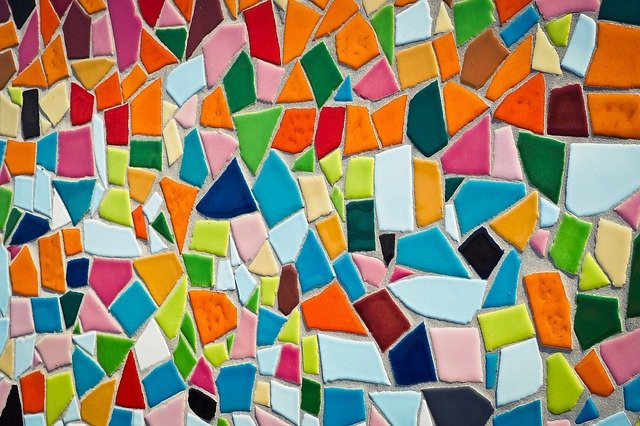
\includegraphics[scale=1.3]{pics/mosaic.jpg}}
		\caption{Mosaikbild (www.pixabay.com,\\ Fotograf: Michael Gaida)}
	\end{subfigure}\hfill
	\begin{subfigure}[t]{0.49\textwidth}
		\centering
		\boxed{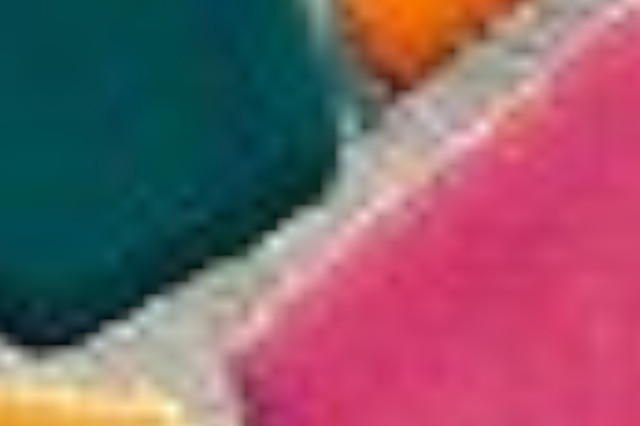
\includegraphics[scale=1.3]{pics/mosaic-zoom-20.jpg}}
		\caption{Mosaikbild bei 20-facher Vergrößerung}
	\end{subfigure}
	\caption{Bildskalierung unter Anwendung bilinearer Interpolation}
	\label{fig:MosaicNearestNeighbor}
\end{figure}
\noindent\textbf{Bikubische Interpolation}
\\\\
Während bei der Linearen Interpolation (siehe Seite \pageref{par:LinearInterpol}) nur jeweils 4 Pixel zur Berechnung eines beliebigen Pixels im Ausgangsbild ausreichen, ist es bei der bikubischen Interpolation nicht ganz so einfach. Der Grund dafür ist, das  auch die Farbkanalgradienten mit in die Berechnung einbezogen werden. 
%\begin{figure}[H]
%	\centering
%	\begin{tikzpicture}[x=0.75pt,y=0.75pt,yscale=-1,xscale=1, scale=0.8, 
%	every node/.style={scale=0.8}]
%		\path (0,200); %set diagram left start at 0, and has height of 300
%		
%
%	\end{tikzpicture}
%	\caption{Darstellung der bikubischen Interpolation}
%	\label{fig:BicubicInterpol}
%\end{figure}

\noindent\textbf{Flächenbasierte Interpolation}
\\\\
\noindent\textbf{LANCZOS-Interpolation}


\section{Statistische Versuchsplanung}
\label{sec:MethodenStatAnalyse}



\chapter{Ausgangssituation}
\label{ch:Ausgangssituation}

\section{Metallographie und Analytik}
\label{sec:MetallographieAnalytik}

\subsection{Lichtmikrokopie für die Erstellung von Bildproben}
\label{subsec:Lichtmikroskopie}

\subsection{Bildmaterial}
\label{subsec:Bildmaterial}

\section{Bestimmung der Mikrostruktur von Gusseisen mit AMGuss}
\label{sec:BestimmungMikrostrukturAMGuss}

\subsection{Kalibrierung}
\label{subsec:Kalibrierung}

\subsection{Erstellung eines Anordnungsklassifikators für die Lamellengraphit-Auswertung}
\label{subsec: ErstellungAnordnungsklassifAMGuss}
Werden Gusseisenwerkstoffe mit Lamellengraphit nach DIN EN ISO 945-1 untersucht, müssen die darin enthaltenen Graphitbestandteile nach dem Beizeichnungssystem für die Klassifizierung von Graphit in Gusseisen klassifiziert  werden \cite{ISO945}. Grundlage für eine solche Klassifizierung sind die in der Norm angegebenen Richtreihenbilder für die Graphitanordnung, wonach insgesamt 5 verschiedene Anordnungsklassen unterschieden werden. Diese sind in der folgenden Abbildung \ref{fig:Anordnungsklassen}} wiedergegeben.

\begin{figure}[H]
	\centering
	\boxed{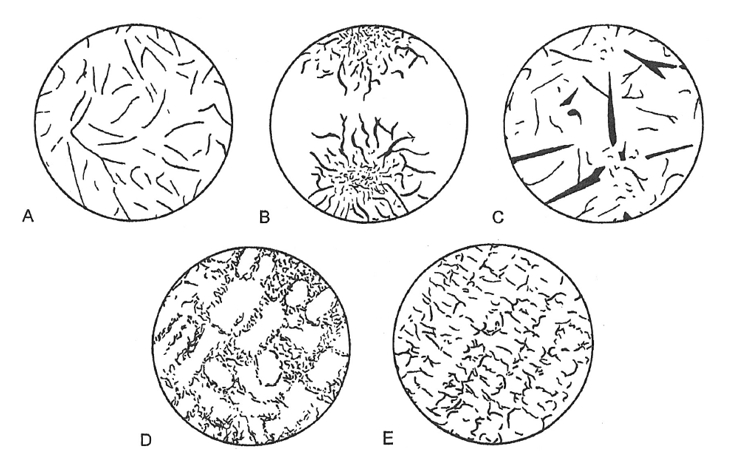
\includegraphics[scale=0.7]{pics/Anordnungsklassen}}
	\caption{Anordnungsklassen A-E (Form \uproman{1}) nach DIN EN ISO 945-1}
	\label{fig:Anordnungsklassen}
\end{figure}

\noindent Zur Durchführung einer Lamellenguss-Auswertung mit AMGuss ist es erforderlich, manuell einen Anordnungsklassifikator zu erstellen. Dafür stellt das Programm dem Nutzer eine entsprechende Funktionalität bereit (Abbildung \ref{fig:ErstAnordnungsklass}).

\begin{figure}[H]
	\centering
	\boxed{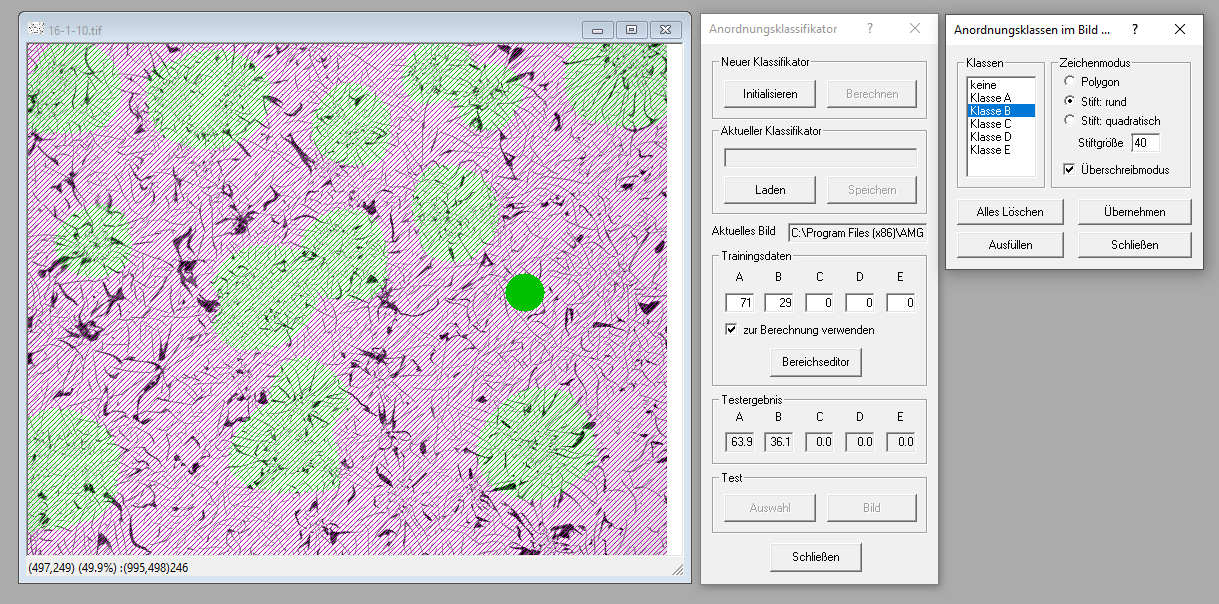
\includegraphics[scale=1.8]{pics/ErstAnordnungsklass}}
	\caption{Erstellung eines Anordnungsklassifikators in AMGuss}
	\label{fig:ErstAnordnungsklass}
\end{figure}



\subsection{Methoden zur Bestimmung der Anordnungstypen A-E von Lamellengraphit}
\label{subsec:AnordnungstypenLamellengraphit}

\subsection{Bewertungsergebnisse einer Lamellengraphit-Auswertung}
\label{subsec:ErgebnisseAMGuss}

\section{Problemstellung}
\label{sec:Problemstellung}

Bei einem allgemeingültigen Anordnungsklassifikator müsste der Nutzer lediglich die Kalibrierung angeben, mit der die Probenbilder aufgenommen wurden und das System wäre in der Lage, die Kalibrierung der Bilder automatisch an die eines im System hinterlegten Klassifikators durch Skalierung anzupassen. Somit würde der Arbeitsschritt, Klassifikatoren manuell erstellen und  verwalten zu müssen, entfallen. Fehler könnten dadurch vermieden und eine Einheitlichkeit der Messungen sichergestellt werden.

\chapter{Konzept}
\label{ch:Konzept}

\section{Sollzustand/Anforderungen}
\label{sec:DefAnforderungenAnordnKlas}
Die Vorgehensweise zur Erstellung eines Anordnungsklassifikators in Kapitel \ref{subsec: ErstellungAnordnungsklassifAMGuss} bereits beschrieben. Dies ist für den Nutzer mit einem nicht unerheblichen Aufwand verbunden. Hinzu kommt eine gewisse Fehleranfälligkeit, da für jede Messung der in Bezug auf die Bildkalibrierung richtige Klassifikator für die Messung ausgewählt werden muss.
\\\\
\noindent Das Gütekriterium an einen solchen Klassifikator ist, die durch Skalierung (bzw. Interpolation) hervorgerufenen und in Kapitel \ref{sec:Problemstellung} bereits näher beschriebenen Messfehler auf ein \textbf{tolerierbares} Maß hin zu minimieren. Allerdings gibt es jedoch, nach den aktuellen allgemein anerkannten Regeln der Technik (vgl. dazu \textcolor{blue}{auf Norm verweisen}) keinen eindeutigen objektiven Maßstab, der zur Beurteilung angelegt werden könnte. Stattdessen beruht die Graphitklassifizierung auf einer visuellen Einschätzung der Spezialisten, welche die Beurteilung der Proben vornehmen. Die Norm DIN ISO 945-1 definiert dabei die Grundlagen, auf denen eine solche Beurteilung zu erfolgen hat. Was also als noch tolerierbar gilt, entscheidet der versierte Nutzer in gewissen Grenzen selbst und wie die Erfahrungen zeigen, existieren teils nicht unerhebliche Abweichungen bei der Einschätzung. 

\section{Erzeugung von Bildern mit unterschiedlichen Ausgangskalibrierungen}


\section{Statistische Versuchsplanung}


\noindent\textcolor{red}{todo:  beschreiben...}  

\subsection{Systemanalyse}
Die Aufgabe, einen allgemeingültigen Anordnungsklassifikator zu entwickeln, der die beschriebenen Anforderungen erfüllt, ist im Grunde die Lösung eines Optimierungsproblems. Dabei ist es erforderlich zu untersuchen, welche Abhängigkeiten zwischen den \textbf{Einflussgrößen} und Zielgrößen zu bestehen, was zunächst vereinfacht in Abbildung dargestellt is.
       
\begin{figure}[H]
	\centering
	\begin{tikzpicture}[x=0.75pt,y=0.75pt,yscale=-1,xscale=1, scale=0.7, every node/.style={scale=0.7}]
		%uncomment if require: \path (0,222); %set diagram left start at 0, and has height of 222
		
		%Flowchart: Process [id:dp31407792865997985] 
		\draw  [fill={rgb, 255:red, 155; green, 155; blue, 155 }  ,fill opacity=0.45 ][line width=2.25]  (147,92) -- (356,92) -- (356,186.35) -- (147,186.35) -- cycle ;
		%Right Arrow [id:dp008081388677440904] 
		\draw  [fill={rgb, 255:red, 248; green, 231; blue, 28 }  ,fill opacity=1 ][line width=1.5]  (199,14) -- (199,56) -- (209,56) -- (189,84) -- (169,56) -- (179,56) -- (179,14) -- cycle ;
		%Right Arrow [id:dp584717372432416] 
		\draw  [fill={rgb, 255:red, 248; green, 231; blue, 28 }  ,fill opacity=1 ][line width=1.5]  (315,14) -- (315,56) -- (325,56) -- (305,84) -- (285,56) -- (295,56) -- (295,14) -- cycle ;
		%Right Arrow [id:dp8933598607947869] 
		\draw  [fill={rgb, 255:red, 184; green, 233; blue, 134 }  ,fill opacity=1 ][line width=1.5]  (70,130) -- (112,130) -- (112,120) -- (140,140) -- (112,160) -- (112,150) -- (70,150) -- cycle ;
		%Right Arrow [id:dp43249460780861937] 
		\draw  [fill={rgb, 255:red, 184; green, 233; blue, 134 }  ,fill opacity=1 ][line width=1.5]  (363,129) -- (405,129) -- (405,119) -- (433,139) -- (405,159) -- (405,149) -- (363,149) -- cycle ;
		%Shape: Rectangle [id:dp02676070817238141] 
		\draw  [line width=3.75]  (5.68,-39.65) -- (514.68,-39.65) -- (514.68,210.35) -- (5.68,210.35) -- cycle ;
		
		% Text Node
		\draw (156,-24) node [anchor=north west][inner sep=0.75pt]  [font=\normalsize] [align=left] {{\scriptsize \textbf{Steuergrößen }}};
		% Text Node
		\draw (278,-24) node [anchor=north west][inner sep=0.75pt]   [align=left] {{\scriptsize \textbf{Störgrößen}}};
		% Text Node
		\draw (266,224.4) node [anchor=north west][inner sep=0.75pt]    {$ $};
		% Text Node
		\draw (151,-6.6) node [anchor=north west][inner sep=0.75pt]  [font=\scriptsize]  {$\{x_{1} ,\ x_{2} ,\ ...,\ x_{n}\}$};
		% Text Node
		\draw (267,-6.6) node [anchor=north west][inner sep=0.75pt]  [font=\scriptsize]  {$\{v_{1} ,\ v_{2} ,\ ...,\ v_{n}\}$};
		% Text Node
		\draw (439,127) node [anchor=north west][inner sep=0.75pt]  [font=\scriptsize] [align=left] {\textbf{Zielgrößen}};
		% Text Node
		\draw (439,137.4) node [anchor=north west][inner sep=0.75pt]  [font=\scriptsize]  {$y_{1} ,\ y_{2} ,\ ...,\ y_{3}$};
		% Text Node
		\draw (13,136) node [anchor=north west][inner sep=0.75pt]  [font=\scriptsize] [align=left] {\textbf{Eingaben}};
		% Text Node
		\draw (177,129) node [anchor=north west][inner sep=0.75pt]  [font=\scriptsize] [align=left] {\begin{minipage}[lt]{108.95844000000001pt}\setlength\topsep{0pt}
				\begin{center}
					\textbf{Versuchsraum}\\\textbf{Ursache-/Wirkunsbez.}
				\end{center}
		\end{minipage}};
	\end{tikzpicture}
	\caption{Usache-/Wirkungsbeziehungen als Black-Box-Modell}
\end{figure}


\subsection{Definition der Zielgrößen}

\textcolor{blue}{Hinweis: Mehrgrößenoptimierungsproblem $\to$ Kombination der Einzelwerte zu einer gewichteten Summe...}

xyxyyxxxy

\subsection{Definition der Einflussgrößen}

\subsection{Modellbildung}

\subsection{Versuchsplanaufbau}

\section{Untersuchung der Auswirkungen von Bildskalierungen auf die Reproduzierbarkeit von Messergebnissen unter Anwendung verschiedener Interpolationsverfahren}

\subsection{Messung der Bilder mit AMGuss vor und nach der Skalierung}

\subsection{Anwendung \textit{einstufiger} Skalierungen auf die erzeugten Bilder}

\subsection{Anwendung \textit{mehrstufiger} Skalierungen auf die erzeugten Bilder}


\chapter{Umsetzung}

\section{Rahmenbedingungen}

\subsection{Technologie-Stack}

\section{Implementierung}

\subsection{Modellierung und algorithmische Beschreibung der Implementierung}

\section{Verwendung von Bildern mit verschiedenen Ausgangskalibrierungen}

\section{Skalierung der erzeugten Bilder (einstufig/mehrstufig)}

\subsection{Bilineare Interpolation}

\subsection{Bikubische Interpolation}

\subsection{Flächenbasierte Interpolation}

\subsection{Nearest-Neighbor-Interpolation}

\subsection{LANCZOS-Interpolation}



\chapter{Evaluierung}

\section{Vergleich angewendeten Interpolationsverfahren}

\subsection{Laufzeitkomplexität und Performance}

\subsection{Kennzahlenvergleich und Interpretation}

\chapter{Zusammenfassung und Auswertung}

\section{Zusammenfassung}

\section{Auswertung}


\bibliographystyle{IEEEtran}
\bibliography{literature}



\end{document}